\documentclass[12pt]{article}

\usepackage{epsf}
\usepackage{graphicx}
\usepackage{psfrag}
\usepackage{amsfonts,amstext,amsmath,amssymb}
\usepackage{hyperref}

%%%%%%%%%%%%%%%%%%%%%%%%%%%%%%%%%%%%%%%%%%%%%%%%%%%%%%%%%%%%%%%%%%%%%
% Diverses commandes
\def\P{{\Bbb P}}
\def\Z{{\Bbb Z}}
\def\R{{\Bbb R}}
\def\N{{\Bbb N}}
\def\F{{\Bbb F}}
\def\Q{{\Bbb Q}}
\def\U{{\Bbb U}}
\def\E{{\Bbb E}}
\newcommand{\NN}{{\cal N}}

\newcommand{\argmin}{\mathop{\mathrm{argmin}}}
\newcommand{\argmax}{\mathop{\mathrm{argmax}}}
\newcommand{\trace}{\mathop{\mathrm{Tr}}}
\newcommand{\diag}{\mathop{\mathrm{diag}}}
\newcommand{\mix}{\textsc{mixmod}}
\newcommand{\II}{1 \! \! 1}
\newcommand{\IR}{\mathbb{R}}
\newcommand{\IZ}{\mathbb{Z}}
\newcommand{\IN}{\mathbb{N}}
\newcommand{\IE}{\mathbb{E}}
\newcommand{\mat}[4]{\begin{array}{cc}#1 & #2 \\#3 & #4 \end{array}}
\newcommand{\matb}[4]{\begin{array}{cc}{\bf #1} & {\bf #2} \\{\bf #3} & {\bf #4} \end{array}}
\newcommand{\med}{\mathrm{med}}
\newcommand{\tr}{\mbox{trace}}
\newcommand{\tra}[1]{\mbox{tr}{\bf #1}}
\newcommand{\var}{\mbox{var}}
% Lettre en gras
\newcommand{\ba}{\mathbf{a}}
\newcommand{\bc}{\mathbf{c}}
\newcommand{\bg}{\mathbf{g}}
\newcommand{\be}{\mathbf{e}}
\newcommand{\bp}{\mathbf{p}}
\newcommand{\bu}{\mathbf{u}}
\newcommand{\bx}{\mathbf{x}}
\newcommand{\bX}{\mathbf{X}}
\newcommand{\bZ}{\mathbf{Z}}
\newcommand{\bz}{\mathbf{z}}
\newcommand{\bt}{\mathbf{t}}
\newcommand{\by}{\mathbf{y}}

% Lettre grecque en gras % requiert \usepackage{amsbsy}
\newcommand{\balpha}{\boldsymbol{\alpha}}
\newcommand{\bDelta}{\boldsymbol{\Delta}}
\newcommand{\bepsilon}{\boldsymbol{\epsilon}}
\newcommand{\bGamma}{\boldsymbol{\Gamma}}
\newcommand{\blambda}{\boldsymbol{\lambda}}
\newcommand{\bmu}{\boldsymbol{\mu}}
\newcommand{\bpi}{\boldsymbol{\pi}}
\newcommand{\bphi}{\boldsymbol{\phi}}
\newcommand{\brho}{\boldsymbol{\rho}}
\newcommand{\btheta}{\boldsymbol{\theta}}
\newcommand{\bTheta}{\boldsymbol{\Theta}}
\newcommand{\bvarepsilon}{\boldsymbol{\varepsilon}}
%%%%%%%%%%%%%%%%%%%%%%%%%%%%%%%%%%%%%%%%%%%%%%%%%%%%%%%%%%%%%%%%%%%%%%%%%%%%%%%%%%%%%%%%%%

\title{{\sc mixmod} Statistical Documentation}
\date{February 10, 2016}

%%%%%%%%%%%%%%%%%%%%%%%%%%%%%%%%%%%%%%%%%%%%%%%%%%%%%%%%%%%%%%%%%%%%%%%%%%%%%%%%%%%%%%%%%%%
%%%%%%%%%%%%%%%%%%%%%%%%%%%%%%%%%%%%%%%%%%%%%%%%%%%%%%%%%%%%%%%%%%%%%%%%%%%%%%%%%%%%%%%%%%%
%%%%%%%%%%%%%%%%%%%%%%%%%%%%%%%%%%%%%%%%%%%%%%%%%%%%%%%%%%%%%%%%%%%%%%%%%%%%%%%%%%%%%%%%%%%
\begin{document}
\maketitle
\tableofcontents
\newpage
\section{Introduction}
Finite mixture models is a powerful tool for density estimation, cluster analysis and
discriminant analysis. {\sc mixmod} is a software for {\sc mix}ture {\sc mod}elling which
considered those three different aspects of mixtures and gives great place to the multivariate
context. In its present version, {\sc mixmod} is dealing with multivariate Gaussian mixture
models for quantitative data, with multivariate multinomial mixture models for categorical data and with combined multivariate Gaussian-multinomial mixture models for mixed quantitative and categorical data.
Basing cluster or discriminant analysis on Gaussian mixture models is a classical and powerful
approach since Gaussian models are useful both for understanding and suggesting powerful
clustering criteria. One of the originality of {\sc mixmod} is to consider a parameterization
of the variance matrix of a cluster through its eigenvalue decomposition leading to many
meaningful models for clustering and classification.  In the same manner, different more or
less parsimonious parameterizations are entering in the multinomial mixture models. Combining both the mixed case quantitative/categorical beneficits from both advantages.

This documentation is organized as follows. In Section 2, the general setting of finite mixture
modelling is sketched. In Section 3, the different available algorithms in {\sc mixmod} for
estimating mixture parameters are presented. In Section 4, the possible strategies for using
{\sc mixmod} algorithms and for initiating them are described. Moreover criteria to select a
model are presented. Section 5 is devoted to the detailed presentation of the Gaussian mixture
models considered in {\sc mixmod} and to a mixture of factor analyser models useful to treat
high dimensional supervised classification problems. Section 6 is devoted to the detailed
presentation of multivariate multinomial mixture models. Section~7  is devoted to the detailed presentation of multivariate combined Gaussian-multivariate mixture models.


%%%%%%%%%%%%%%%%%%%%%%%%%%%%%%%%%%%%%%%%%%%%%%%%%%%%%%%%%%%%%%%%%%%%%%%%%%%%%%%%%%%%%%%%%%%%%%%%%%%
%%%%%%%%%%%%%%%%%%%%%%%%%%%%%%%%%%%%%%%%%%%%%%%%%%%%%%%%%%%%%%%%%%%%%%%%%%%%%%%%%%%%%%%%%%%%%%%%%%%
%%%%%%%%%%%%%%%%%%%%%%%%%%%%%%%%%%%%%%%%%%%%%%%%%%%%%%%%%%%%%%%%%%%%%%%%%%%%%%%%%%%%%%%%%%%%%%%%%%%
\section{Mixture model}
Let ${\bf x}=\{ {\bf x}_1,...,{\bf x}_n\}$ be $n$ independent vectors in ${\mathcal X}$ such that each
${\bf x}_i$ arises from a probability distribution with density
\begin{eqnarray}
  f({\bf x}_i|\theta) = \sum_{k=1}^K p_k h({\bf x}_{i}|
\blambda_{k})
\end{eqnarray}
where the $p_k$'s are the mixing proportions ($0<p_k<1$ for all $k=1,...,K$ and
$p_1+...+p_K=1$), $h(\cdot| \blambda_{k})$ denotes a $d$-dimensional distribution parameterized
by $\blambda_k$. As we will see in Section 5, $h$ is for instance the density of a Gaussian
distribution with ${\mathcal X}=\IR^d$, mean $\bmu$ and variance matrix $\Sigma$ and thus, $\blambda=(\bmu, \Sigma)$.

It is worth noting that for a mixture distribution, a sample of indicator vectors or {\em
  labels} ${\bf z}=\{ {\bf z}_1,...,{\bf z}_n\}$, with ${\bf z}_i=(z_{i1},\ldots,z_{iK})$,
$z_{ik}=1$ or 0, according to the fact that ${\bf x}_i$ is arising from the $k$th mixture
component or not, is associated to the observed data ${\bf x}$. The sample ${\bf z}$ can be
{\em known} in which case we are in a discriminant analysis context where the problem is
essentially to predict an indicator vector ${\bf z}_{n+1}$ from a new observed data vector
${\bf x}_{n+1}$. But the sample ${\bf z}$ can be {\em unknown} in which case we are in a
density estimation context or cluster analysis context if the estimation of the ${\bf z}_i$'s
are of primary interest. In each case, the vector parameter to be estimated is
$\theta=(p_1,\ldots,p_K,\lambda_1,\ldots,\lambda_K)$.

%%%%%%%%%%%%%%%%%%%%%%%%%%%%%%%%%%%%%%%%%%%%%%%%%%%%%%%%%%%%%%%%%%%%%%%%%%%%%%%%%%%%%%%%%%%%%%%%%%%
\subsection{Density estimation from a mixture model}
Mixture modelling can be regarded as a flexible way to represent a probability density
function, and thus providing a semi parametric tool for density estimation.  When the labels
${\bf z}$ are unknown, maximum likelihood estimation of mixture models can be performed in {\sc
  mixmod} via the EM algorithm of Dempster, Laird and Rubin (1977) or by a stochastic version
of EM called SEM (see McLachlan and Peel, 2000). In each case, the parameter $\theta$ is chosen
to maximize the observed log-likelihood
\begin{equation}
  \label{eq:vraisemblance}
  L(\theta|\bx_1,\ldots,\bx_n)=\sum_{i=1}^n \ln \left(\sum_{k=1}^K p_k h(\bx_i,\blambda_k)\right).
\end{equation}

%%%%%%%%%%%%%%%%%%%%%%%%%%%%%%%%%%%%%%%%%%%%%%%%%%%%%%%%%%%%%%%%%%%%%%%%%%%%%%%%%%%%%%%%%%%%%%%%%%%
\subsection{Clustering with mixture model}
Cluster analysis is concerned with discovering a group structure in a $n$ by $d$ data matrix
$\bx=\{\bx_1,...,\bx_n\}$ where $\bx_i$ is an individual in ${\mathcal X}$. Consequently, the result
provided by clustering is typically a partition of $\bx$ into $K$ groups defined with the
labels $\tilde\bz=\{\tilde\bz_1,...,\tilde\bz_n\}$, with $\tilde\bz_i=(\tilde
z_{i1},\ldots,\tilde z_{iK})$, $\tilde z_{ik}=1$ or 0 according to $\bx_i$ is assigned to the
$k$th group or not.

Many authors have considered non hierarchical clustering methods in which a mixture of
distributions is used as a statistical model. In this context, two commonly used maximum
likelihood (m.l.) approaches have been proposed: the mixture approach and the classification
approach. Loosely speaking, the mixture approach is aimed to maximize the likelihood over the
mixture parameters, whereas the classification approach is aimed to maximize the likelihood
over the mixture parameters and over the mixture component labels.

\subsubsection{The mixture approach}
In this approach, a partition of the data can directly be derived from the m.l. estimates
$\hat{\theta}$ of the mixture parameters obtained, for instance, by the EM or the SEM algorithm
described hereafter, by assigning each ${\mathbf x}_{i}$ to the component providing the largest
conditional probability that ${\mathbf x}_{i}$ arises from it using a MAP (Maximum A
Posteriori) principle.  Denoting $\bz_i$ the label of $\bx_i$, the MAP principle is as follows
\begin{equation}
  \tilde z_{ik} =
  \left\{\begin{array}{l}
      1 \mbox{ if } k = \arg\max_{\ell=1\ldots,K}
      t_{\ell}(\bx_i|\hat\theta)\\
      0 \mbox{ if not}
    \end{array}\right.
\end{equation}
where
$$t_k(\bx_i|\hat\theta)=\frac{\hat p_k h(\bx_i|\hat\blambda_k)} {\sum_{\ell=1}^K \hat p_\ell
  h(\bx_i|\hat \blambda_\ell)}.$$

\subsubsection{The classification approach}
The second approach available in {\sc mixmod} is the classification approach.  In this
approach, the indicator vectors ${\bf z}=\{ {\bf z}_1,...,{\bf z}_n\}$, identifying the mixture
component origin, are treated as unknown parameters. The Classification Maximum Likelihood
(c.m.l.) method is used to estimate both the parameters $\theta$ and ${\bf z}$.  The
classification likelihood criterion is defined by
\begin{equation} \label{cl}
  CL(\theta, {\bf z}_{1},\ldots,{\bf z}_{n}|{\bf
    x}_{1},\ldots,{\bf x}_{n}) = \sum_{i=1}^n\sum_{k=1}^{K}
  z_{ik}\ln[p_{k} h({\bf x}_i|\blambda_k)].
\end{equation}
The $CL$ criterion can be maximized by making use of a classification version of the EM
algorithm, the so-called CEM algorithm (Celeux and Govaert 1992) which includes a
classification step (C-step) between the E and M steps.

%%%%%%%%%%%%%%%%%%%%%%%%%%%%%%%%%%%%%%%%%%%%%%%%%%%%%%%%%%%%%%%%%%%%%%%%%%%%%%%%%%%%%%%%%%%%%%%%%%%
\subsection{Discriminant Analysis}
When the labels ${\bz}$ are known, we are concerned with discriminant analysis: in discriminant
analysis, data are composed by $n$ observations $\bx=(\bx_1,...,\bx_n\}$ $(\bx_i \in \IR^d)$
and a partition of $\bx$ into $K$ groups defined with the labels $\bz=\{\bz_1,...,\bz_n\}$. The
aim is to estimate the group $\bz_{n+1}$ of any new individual $\bx_{n+1}$ of $\IR^d$ with
unknown label.

In this context, the $n$ couples $(\bx_i,\bz_i)$,..., $(\bx_n,\bz_n)$ are realizations of $n$
identically and independently distributed random vectors $(\bX_i,\bZ_i)$,...,$(\bX_n,\bZ_n)$.
The distribution of each $(\bX_i,\bZ_i)$ ($1\leq i\leq n$) is
\begin{eqnarray}
  f(\bx_i,\bz_i|\theta) = \prod_{k=1}^K p_k^{z_{ik}}[h(\bx_i| \blambda_k)]^{z_{ik}},
\end{eqnarray}
where $p_k$ is the prior probability of the $k$th group (the mixing proportion), $h(\bx_i|
\blambda_k)$ is a probability density with parameters $\blambda_k$ and the whole parameter is
$\theta=(p_1,\ldots,p_{K},\blambda_1,\ldots,\blambda_K)$.

An estimate $\hat\theta$ of $\theta$ is obtained by the m.l. method
\begin{equation}
  \hat\theta = \arg\max\limits_{\theta}L(\theta|\bx,\bz)
\end{equation}
where the log-likelihood function $L(\theta|\bx,\bz)$ is defined by
\begin{equation}
  L(\theta|\bx,\bz)=\sum_{i=1}^n\sum_{k=1}^K z_{ik}\ln (p_k h (\bx_i| \blambda_k)).
\end{equation}
This estimate $\hat\theta$ allows to assign any new point $\bx_{n+1}$ with unknown membership
in one of the $K$ groups by the maximum a posteriori (MAP) procedure. Computing the conditional
probability $t_k(\bx_{n+1}|\hat\theta)$ that $\bx_{n+1}$ arises from the $k$th group
\begin{equation}
  t_k(\bx_{n+1}|\hat\theta)=\frac{\hat p_k h (\bx_{n+1}|\hat\blambda_k)}
  {\sum_{\ell=1}^K \hat p_\ell h (\bx_{n+1}|\hat\blambda_\ell)},
\end{equation}
the MAP procedure consists of assigning $\bx_{n+1}$ to the group maximizing this conditional
probability, i.e.
\begin{equation}
  \hat z_{n+1\;k} = \left\{\begin{array}{l}
  1 \mbox{ if } k = \arg\max_{\ell=1\ldots,K}
  t_{\ell}(\bx_{n+1}|\hat\theta)\\
  0 \mbox{ if not}
  \end{array}\right..
\end{equation}
% where we recall that $\bz_i \in \{1,\ldots,K\}$ is the group index of $\bx_i$.


%%%%%%%%%%%%%%%%%%%%%%%%%%%%%%%%%%%%%%%%%%%%%%%%%%%%%%%%%%%%%%%%%%%%%%%%%%%%%%%%%%%%%%%%%%%%%%%%%%%
%%%%%%%%%%%%%%%%%%%%%%%%%%%%%%%%%%%%%%%%%%%%%%%%%%%%%%%%%%%%%%%%%%%%%%%%%%%%%%%%%%%%%%%%%%%%%%%%%%%
%%%%%%%%%%%%%%%%%%%%%%%%%%%%%%%%%%%%%%%%%%%%%%%%%%%%%%%%%%%%%%%%%%%%%%%%%%%%%%%%%%%%%%%%%%%%%%%%%%%
\section{Algorithms in {\sc mixmod}}
\subsection{EM algorithm}
Starting from an initial arbitrary parameter $\theta^0$, the $m$th iteration of the EM
algorithm consists of repeating the following E and M steps.
\begin{itemize}
\item {\bf E step:} The current conditional probabilities that $z_{ik}=1$ for $i=1,\ldots,n$
  and $k=1,\ldots,K$ are computed using the current value $\theta^{m-1}$ of the parameter:
  \begin{equation}
    \label{eq:condi}
    t^m_{ik}=t^m_k(\bx_i|\theta^{m-1})=\frac{ p^{m-1}_kh (\bx_i|{\blambda^{m-1}_k})}
    {\sum_{\ell=1}^K  p^{m-1}_\ell h(\bx_i|\blambda^{m-1}_\ell)}.
  \end{equation}
\item {\bf M step:} The m.l. estimate $\theta^m$ of $\theta$ is updated using the conditional
  probabilities $t^m_{ik}$ as conditional mixing weights. It leads to maximize
  \begin{equation} \label{eq:proportionEM}
    F(\theta| {\bf x}_{1},\ldots,{\bf x}_{n}, {\bf
      t}^m)=\sum_{i=1}^{n}\sum_{k=1}^{K} t_{ik}^m \ln \left [p_{k} \Phi({\bf
        x}_{i}|\blambda_{k})\right ],
  \end{equation}
  where ${\bf t}^m=(t_{ik}^m, i=1,\ldots,n, k=1,\ldots,K)$. Updated expression of mixture
  proportions are, for $k=1,\ldots,K$,
  \begin{equation}
    p_k^m=\frac{\sum_{i=1}^n t^m_{ik}}{n}.
  \end{equation}
  Detailed formula for the updating of the $\blambda_k$'s are depending of the component
  parameterization $\blambda$ and cannot be detailed here.
\end{itemize}

%%%%%%%%%%%%%%%%%%%%%%%%%%%%%%%%%%%%%%%%%%%%%%%%%%%%%%%%%%%%%%%%%%%%%%%%%%%%%%%%%%%%%%%%%%%%%%%%%%%
\subsection{SEM algorithm}
The SEM algorithm is a stochastic version of EM incorporating between the E and M steps a
restoration of the unknown component labels $\bz_i$, $i=1,\ldots,n,$ by drawing them at random
from their current conditional distribution. Starting from an initial parameter $\theta^0$, an
iteration of SEM consists of three steps.
\begin{itemize}
\item {\bf E step:} The conditional probabilities $t^m_{ik}$ $(1 \leq i \leq n, 1 \leq k \leq
  K)$ are computed for the current value of $\theta$ as done in the E step of EM.
\item {\bf S step:} A partition $P^m=(P^m_1,\ldots,P^m_K)$ of ${\mathbf x}_1,\ldots,{\mathbf
    x}_n$ is designed by assigning each point ${\mathbf x}_i$ at random to one of the mixture
  components according to the multinomial distribution with parameter $(t^m_{ik}, 1 \leq k \leq
  K)$.
\item {\bf M step:} The m.l. estimate of $\theta$ is updated using the cluster $P^m_k$ as
  sub-sample $(1 \leq k \leq K)$ of the $k$th mixture component. This step leads generally to
  simple formula.  For instance,
  \begin{equation}
    p_k^m=\frac{\mbox{card}(P^m_k)}{n}.
  \end{equation}
\end{itemize}

SEM does not converge pointwise.  It generates a Markov chain whose stationary distribution is
more or less concentrated around the m.l. parameter estimator. A natural parameter estimate from
a SEM sequence $(\theta^r)_{r=1, \ldots,R}$ is the mean $\sum_{r=b+1}^R \theta^r/(R-b)$ of the
iterates values where the first $b$ burn-in iterates have been discarded when computing this
mean.  An alternative estimate is to consider the parameter value leading to the highest
likelihood in a SEM sequence.

A remark is to be made. When several observations are associated to the same vector, they are
assigned to the same mixture component in the S step. This choice can make a difference when
concerned with categorical data. It is expected to give a larger influence to the random
assignments.

%%%%%%%%%%%%%%%%%%%%%%%%%%%%%%%%%%%%%%%%%%%%%%%%%%%%%%%%%%%%%%%%%%%%%%%%%%%%%%%%%%%%%%%%%%%%%%%%%%%
\subsection{CEM algorithm}
This algorithm incorporates a classification step between the E and M steps of EM. Starting
from an initial parameter $\theta^0$, an iteration of CEM consists of three steps.
\begin{itemize}
\item {\bf E step:} The conditional probabilities $t^m_{ik}$ $(1 \leq i \leq n, 1 \leq k \leq
  K)$ are computed for the current value of $\theta$ as done in the E step of EM.
\item {\bf C step:} A partition $P^m=(P^m_1,\ldots,P^m_K)$ of ${\mathbf x}_1,\ldots,{\mathbf
    x}_n$ is designed by assigning each point ${\mathbf x}_i$ to the component maximizing the
  conditional probability $(t^m_{ik}, 1 \leq k \leq K)$.
\item {\bf M step:} The m.l. estimates $(\hat{p}_k,\blambda_k)$ are computed using the cluster
  $P_k^m$ as sub-sample $(1 \leq k \leq K)$ of the $k$th mixture component as done in the M
  step of SEM.
\end{itemize}
CEM is a {\em K-means}-like algorithm and contrary to EM, it converges in a finite number of
iterations. CEM is not maximizing the observed log-likelihood $L$ (\ref{eq:vraisemblance}) but
is maximizing in $\theta$ and $\bz_{1},\ldots,\bz_{n}$ the complete data log-likelihood $CL$
(\ref{cl}) where the missing component indicator vector $\bz_i$ of each sample point is
included in the data set. As a consequence, CEM is not expected to converge to the m.l.
estimate of $\theta$ and yields inconsistent estimates of the parameters especially when the
mixture components are overlapping or are in disparate proportions (see McLachlan and Peel
2000, Section 2.21).

%%%%%%%%%%%%%%%%%%%%%%%%%%%%%%%%%%%%%%%%%%%%%%%%%%%%%%%%%%%%%%%%%%%%%%%%%%%%%%%%%%%%%%%%%%%%%%
%%%%%%%%%%%%%%%%%%%%%%%%%%%%%%%%%%%%%%%%%%%%%%%%%%%%%%%%%%%%%%%%%%%%%%%%%%%%%%%%%%%%%%%%%%%%%%
%%%%%%%%%%%%%%%%%%%%%%%%%%%%%%%%%%%%%%%%%%%%%%%%%%%%%%%%%%%%%%%%%%%%%%%%%%%%%%%%%%%%%%%%%%%%%%
\section{Using {\sc mixmod}}
\subsection{Stopping rules}
In {\sc mixmod} they are three ways to stop an algorithm.
\begin{itemize}
\item An algorithm can be stopped after a pre-defined number of iterations (100 by default in
  {\sc mixmod}). This possibility is available for EM, SEM and CEM.
\item An algorithm can be stopped using a threshold for the relative change of the criterion at
  hand (the likelihood $L$ or the classification likelihood $CL$). This possibility is
  available with EM and CEM.  It is not recommended since EM can encounter slow convergence
  situations and CEM is converging in a finite number of iterations.
\item An algorithm can be stopped at stationarity. Obviously, this possibility is only
  available for CEM.
\end{itemize}

%%%%%%%%%%%%%%%%%%%%%%%%%%%%%%%%%%%%%%%%%%%%%%%%%%%%%%%%%%%%%%%%%%%%%%%%%%%%%%%%%%%%%%%%%%%%%%
\subsection{Initialization strategies}
The solution provided by EM can highly depend on its starting position especially in a
multivariate context. Thus, it is important to have sensible ways for initiating EM to get a
sensible optimum of the likelihood. Obviously, in some cases it is possible to start from a
particular partition of the data or from a pre-defined $\theta^0$ and those initializations of
EM are possible in {\sc mixmod}. But there is the need to have more general strategies. In {\sc
  mixmod}, it is possible to easily link the algorithms EM, SEM and CEM in all imaginable ways.
Thus, in Biernacki {\it et al.} (2003), we have experimented an efficient three step
Search/Run/Select (S/R/S) strategy for maximizing the likelihood:
\begin{enumerate}
\item Build a search method for generating $p$ initial positions. This could be based on random
  starts or the output from an algorithm like a Classification EM (CEM) algorithm, a Stochastic
  EM (SEM) algorithm or short runs of the standard EM algorithm. The parameter $p$ is depending
  on an allotment of iterations.
\item Run the EM algorithm a set number of times at each initial position with a fixed number
  of iterations.
\item Select the solution providing best likelihood among the $p$ trials, say $\theta^*$.
\end{enumerate}
This three-step strategy can be compounded by repeating the three steps $x$ times and using the
$\theta_1^*,\ldots,\theta_x^*$ as the starting positions in step 1. By compounding, one
increases starting position variation, but one must decrease the length of the EM runs possible
within the steps in order to fix the total number of steps.

Possible variants of this strategy are now described.
\paragraph{Random initialization} Usually this random initial position is obtained by drawing
at random component means in the data set. Since this is probably the most employed way of
initiating EM, it can be regarded as a reference strategy. An extension of this simple strategy
consists of repeating it $x$ times from different random positions and selecting the solution
maximizing the likelihood among those $x$ runs. This ``$x$EM'' strategy is the basic S/R/S
algorithm.

\paragraph{Using the CEM algorithm}
Runs of CEM from random positions followed by EM from the position providing the highest {\it
  complete} data log-likelihood obtained with CEM. And, $x$ repetitions of the previous
strategy give rise to an additional strategy denoted ``$x$CEM-EM''.

\paragraph{Using short runs of EM}
By a short run of EM, we mean that we do not wait for convergence and that we stop the
algorithm as soon as
\begin{equation} \label{seuil}
  \frac{L^m-L^{m-1}}{L^m-L^0} \leq 10^{-2},
\end{equation}
$L^m$ denoting the observed log-likelihood at $m$th iteration.  Here $10^{-2}$ represents a
threshold value which has to be chosen on a pragmatic ground. It leads to the following
strategies : several short runs of EM from random positions followed by a long run of EM from
the solution maximizing the {\it observed} log-likelihood. And, $x$ repetitions of the previous
strategy lead to the so called ``$x$em-EM'' strategy.

\paragraph{Using Stochastic EM}
The stochastic EM algorithm generates an ergodic Markov chain.  Thus a sequence of parameter
estimates via SEM is expected to visit the whole parameter space with long sojourns in the
neighborhood of sensible maxima of likelihood functions. This characteristic of SEM leads to
the following strategies.
\begin{itemize}
\item ``SEMmean-EM'': A run of SEM, followed by a run of EM from the solution obtained by
  computing the mean values of the sequence of parameter estimates provided by SEM after a
  burn-in period.  The idea underlying this strategy is that SEM is expected to spend most of
  the time near sensible likelihood maxima with a large attractive neighborhood.
\item ``SEMmax-EM'': The {\em same} run of SEM followed by a run of EM from the position
  leading to the highest maximum likelihood value reached by SEM.  Here, the idea is that a SEM
  sequence is expected to enter rapidly in the neighborhood of the global maximum of the
  likelihood function.
\end{itemize}
It is difficult to recommend a particular strategy among the ones presented above.  However,
the strategy ``$x$em-EM'' gives generally good performances and is the default strategy in {\sc
  mixmod}.

%%%%%%%%%%%%%%%%%%%%%%%%%%%%%%%%%%%%%%%%%%%%%%%%%%%%%%%%%%%%%%%%%%%%%%%%%%%%%%%%%%%%%%%%%%%%%%
\subsection{Criteria to select a model}
It is of high interest to automatically select a model and the number $K$ of mixture
components.  However, choosing a sensible mixture model is highly dependent of the modelling
purpose.

In {\sc mixmod}, two criteria are proposed in a supervised setting: BIC and cross-validation.
In an unsupervised setting, three criteria are available: BIC, ICL and NEC. In a density
estimation perspective, BIC must be preferred. But in a cluster analysis perspective, ICL and
NEC can provide more parsimonious answers. Nevertheless, NEC is essentially devoted to choose
the number of mixture components $K$, rather than the model parameterization. Before describing
those criteria, it can be noted that if no information on $K$ is available, it is recommended
to vary it between 1 and the smallest integer larger than $n^{0.3}$ (see Bozdogan 1993).

\subsubsection{The Bayesian Information Criterion (BIC)}
A finite mixture model is characterized by the number of components $K$ and the vector
parameter $\theta=(p_1,\ldots,p_K,\blambda_1,\ldots,\blambda_K)$. A classical way of choosing
a model is to select this one maximizing the integrated likelihood,
\begin{equation}
  (\hat m, \hat K) = \mbox{arg} \max_{m,K} {\mathbf f}({\mathbf x}\mid m,K)
\end{equation}
where the integrated likelihood is
\begin{equation} \label{il}
  {\mathbf f}({\mathbf x} \mid m,K)=\int_{\Theta_{m,K}}{\mathbf
    f}({\mathbf x} \mid m,K,\theta) \pi(\theta \mid m,K) d\theta,
\end{equation}
with the likelihood
\begin{equation}
  {\mathbf f}({\mathbf x} \mid m,K,\theta)=\prod_{i=1}^{n}f({\mathbf x}_i \mid m,K,\theta),
\end{equation}
and $\Theta_{m,K}$ being the parameter space of the model $m$ with $K$ components and
$\pi(\theta \mid m,K)$ a non informative or a weakly informative prior distribution on $\theta$
for this model. An asymptotic approximation of the integrated likelihood, valid under
regularity conditions, has been proposed by Schwarz (1978)
\begin{equation}
  \log{\mathbf f}({\mathbf x} \mid m,K) \approx \log {\mathbf
    f}({\mathbf x} \mid m, K,\hat \theta)-\frac{\nu_{m,K}}{2} \log (n),
\end{equation}
where $\hat\theta$ is the m.l. estimate of $\theta$
\begin{equation}
  \hat\theta= \arg \max_{\theta} {\mathbf f}({\mathbf x} \mid m,K,\theta)
\end{equation}
and $\nu_{m,K}$ is the number of free parameters in the model $m$ with $K$ components. It leads
to minimize the so-called BIC criterion
\begin{equation} \label{eq:bic}
  \mbox{BIC}_{m,K}=-2L_{m,K}+\nu_{m,K}\ln n,
\end{equation}
where $L_{m,K} = \log {\mathbf f}({\mathbf x} \mid m, K,\hat \theta)$ is the maximum
log-likelihood for $m$ and $K$.  Despite the fact that those regularity conditions are not
fulfilled for mixtures, it has been proved that the criterion BIC is consistent (Keribin 2000)
and has been proved to be efficient on a practical ground (see for instance Fraley and Raftery
1998).

\subsubsection{The Integrated Completed Likelihood (ICL)}
The use of the integrated likelihood (\ref{il}) does not take into account the ability of the
mixture model to give evidence for a clustering structure of the data.  An alternative is to
consider the integrated likelihood of the complete data $({\mathbf x}, {\mathbf z})$ (or
integrated completed likelihood) (Biernacki {\it et al.} 2000)
\begin{equation} \label{cil}
  {\mathbf f}({\mathbf x}, {\mathbf z} \mid
  m,K)=\int_{\Theta_{m,K}}{\mathbf f}({\mathbf x}, {\mathbf z} \mid
  m,K,\theta) \pi(\theta \mid m,K) d\theta,
\end{equation}
where
\begin{equation}
  {\mathbf f}({\mathbf x}, {\mathbf z} \mid m,K,\theta)=
  \prod_{i=1}^n f({\mathbf x}_i,{\mathbf z}_i \mid m,K,\theta)
\end{equation}
with
\begin{equation}
  f({\mathbf x}_i,{\mathbf z}_i \mid m,K,\theta)= \prod_{k=1}^K
  p_k^{z_{ik}}\left[h({\mathbf x}_i \mid {\blambda}_k)\right]^{z_{ik}}.
\end{equation}
This integrated completed likelihood can be approximated from a BIC-like approximation.
That is
\begin{equation}
  \log {\mathbf f}({\mathbf x},{\mathbf z} \mid m,K)\approx \log
  {\mathbf f}({\mathbf x},{\mathbf z} \mid m,K,\hat\theta^{*}) -
  \frac{\nu_{m,K}}{2} \log n
\end{equation}
where
\begin{equation} \label{mvc}
  \hat \theta^{*}=\arg \max_{\theta} {\mathbf f}({\mathbf
    x},{\mathbf z} \mid m,K,\theta).
\end{equation}
But ${\mathbf z}$ is unknown. It means that the objective functions to be maximized in
(\ref{cil}) and (\ref{mvc}) are not available and so is $\hat\theta^{*}$. However, for $n$
large enough, $\hat \theta^{*}$ can be approximated by the m.l. estimator
$\hat\theta$. Moreover, the missing data ${\mathbf z}$ can be replaced using the MAP principle:
$\mathbf {\tilde z}=\mbox{MAP}(\hat \theta)$. It leads finally to the ICL criterion to be
minimized (Biernacki {\it et al.}  2000)
\begin{equation} \label{icl}
  \mbox{ICL}_{m,K}= -2\log {\mathbf f}({\mathbf x}, \tilde {\mathbf
    z} \mid m,K,\hat \theta) + \nu_{m,K} \log n,
\end{equation}
that we can also write as a BIC criterion penalized by an entropy term:
\begin{equation} \label{icl2}
  \mbox{ICL}_{m,K}= \mbox{BIC}_{m,K} - 2\sum_{i=1}^n\sum_{k=1}^K
  \tilde z_{ik}\ln t_{ik}.
\end{equation}
% Note that $\hat\theta$ may be also the c.m.l. estimator if only this one is available.

\subsubsection{The Normalized Entropy Criterion (NEC)}
This entropy criterion measures the ability of a mixture model to provide well-separated
clusters and is derived from a relation highlighting the differences between the maximum
likelihood (m.l.) approach and the classification maximum likelihood (c.m.l.) approach to the
mixture problem. Recall that NEC is essentially devoted to choose the number of mixture
components $K$, not the model $m$.

We note $\hat\theta$ the m.l. estimator of $\theta$ and
\begin{equation}
  t_{ik} = t_k({\bf x}_i | \hat\theta) = \frac{\hat p_{k}h({\bf
      x}_{i}| \hat{\blambda}_{k})}{\sum_{k'=1}^{K}\hat p_{k'}h({\bf
      x}_{i}| \hat {\blambda}_{k'})}
\end{equation}
the associated conditional probability that ${\bf x}_i$ arises from to the $k$th mixture
component. Direct calculations show that
\begin{equation}
  L_K=C_K+E_K,
\end{equation}
with $L_K$ the maximum log-likelihood,
\begin{equation}
  C_K=\sum_{k=1}^{K}\sum_{i=1}^{n}t_{ik}\mbox{ ln }[\hat
  p_{k}h({\bf x}_{i}|\hat{\blambda}_{k})],
\end{equation}
and
\begin{equation}
  E_K=-\sum_{k=1}^{K}\sum_{i=1}^{n}t_{ik}\mbox{ ln }t_{ik} \geq 0.
\end{equation}
This relation with the fact that the entropy term $E_K$ measures the overlap of the mixture
components (If the mixture components are well-separated $E_K \simeq 0$.  But if the mixture
components are poorly separated, $E_K$ has a large value.) leads to the normalized entropy
criterion (Celeux and Soromenho 1996)
\begin{equation}
  \mbox{NEC}_K=\frac{E_K}{L_K-L_1}
\end{equation}
as a criterion to be minimized for assessing the number of clusters arising from a mixture.

Note that NEC$_1$ is not defined. Biernacki {\em et al.} (1999) proposed the following
efficient rule to deal with this problem.  Let $K^{\star}$ be the value minimizing NEC$_K$,
($2\leq K \leq K_{\mbox{sup}}$), $K_{\mbox{sup}}$ being an upper bound for the number of
mixture components. We choose $K^{\star}$ clusters if NEC$_{K^{\star}}\leq 1$, otherwise we
declare no clustering structure in the data.

\subsubsection{The cross-validation criterion (CV)}
This criterion is valid only in the discriminant analysis (supervised) context.  In this
situation, note that only the model $m$ has to be selected.  Cross validation is a resampling
method which can be summarised as follows: Let $S$ be the whole dataset. Consider random splits
of $S$ into $V$ independent datasets $S_1,\ldots, S_V$ of approximatively equal sizes $n_1,
\ldots, n_V$. (If $n/V$ is an integer $h$, we have $n_1=\ldots=n_V=h$.) The CV criterion is
defined by
\begin{equation}
  \mbox{CV}_m=\frac{1}{n}\sum_{v=1}^V\sum_{i\in S_v} \delta(\hat\bz_i^{(v)},\bz_i)
\end{equation}
with $\delta$ the 0-1 cost and $\hat\bz_i^{(v)}$ denotes the group to which $\bx_i$ is assigned
when designing the assignment rule from the entire data set $(\bx,\bz)$ without $S_v$.  When
$V=1$ the cross validation is known as the {\em leave one out} method, and, in this case, fast
estimation of the $n$ discriminant rules is implemented in the Gaussian situation (Biernacki
and Govaert 1999). In {\sc mixmod}, the default value for the cross validation criterion is
$V=10$.

\subsubsection{The double cross-validation criterion (DCV)}
The CV error rate described above gives an optimistic estimate of the actual error rate because
the method includes the selection of one model among several ones.  Thus, there is a need to
assess the actual error rate from an independent sample. This is the purpose of the DCV
criterion, implemented in \mix{} version 1.7.

%It uses a (randomly selected) part of the dataset to estimate the parameters and to choose the
%best model and the remaining part for the computation of the error-rate. Such procedure
%is repeated several times in order to get an idea of the precision of the computed error rate.

The double cross-validated error rate is computed in \mix{} as follows: Repeat the three
following steps for $v$ in $1,\ldots,V$ with $S^{-}_v = S\ \backslash\ S_v$
\begin{itemize}
\item[$\blacktriangleright$] build the models using the $S^{-}_v$ dataset
\item[$\blacktriangleright$] select the best model regarding the CV criterion: $m^{\star}_v$
\item[$\blacktriangleright$] estimate the error rate $e_v$ of $m^{\star}_v$ using $S_v$
\begin{equation}
  e_v = \frac{1}{n_v} \sum_{i \in S_v} \delta(\hat\bz_i^{m^{\star}_v},\bz_i).
\end{equation}
\end{itemize}
The DCV error rate ($\bar{e}$) is finally obtained by averaging the $e_1,\ldots, e_V$.  The
empirical standard error of the error rate is given by $\sigma_e$
\begin{equation}
  \bar{e} = \frac{1}{V} \sum_{v=1}^V e_v\ \ \ , \ \ \
  \sigma_e  = \left( \frac{1}{V-1} \sum_{v=1}^V (e_v - \bar{e} )^2   \right)^{1/2}.
\end{equation}
Recall that in {\sc mixmod}, the default value of $V$ is 10.

%%%%%%%%%%%%%%%%%%%%%%%%%%%%%%%%%%%%%%%%%%%%%%%%%%%%%%%%%%%%%%%%%%%%%%%%%%%%%%%%%%%%%%%%%%%%%
\subsection{Partial labeling of individuals}
{\sc MIXMOD} allows  partial labeling. Recall that in density estimation or clustering context,
observed data are $\bx=\{ \bx_1,...,\bx_n\}$, the corresponding labels
$\bz=\{\bz_1,...,\bz_n\}$ being unknown.  On the contrary, in the discriminant analysis
context, all the labels $\bz$ are available to estimate the mixture parameter $\theta$.  In
some cases, the following intermediate situation may occur: the set $\bx$ of individuals is
divided into two sets $\bx=(\bx^\ell,\bx^u)$ where ${\bx^\ell}=\{\bx_1,...,\bx_m\}$ ($1\leq m
\leq n$) are units with known labels $\bz^\ell=\{\bz_1,...,\bz_m\}$, and
${\bx^u}=\{\bx_{m+1},...,\bx_n\}$ units with unknown labels $\bz^u=\{\bz_{m+1},...,\bz_n\}$.

The m.l. mixture parameter estimate is derived by maximizing the following log-likelihood
\begin{equation}
  L(\theta | \bx,\bz^\ell) = \sum_{i=1}^m\sum_{k=1}^{K}z_{ik} \ln[p_k
  h(\bx_i|\blambda_k)] + \sum_{i=m+1}^{n} \ln \left( \sum_{k=1}^K
    p_k h(\bx_i|\blambda_k) \right).
\end{equation}

In a clustering context using the classification approach, the c.m.l. method, is maximizing the
following completed log-likelihood
\begin{equation}
  CL(\theta, \bz^u | \bx,\bz^\ell) = \sum_{i=1}^m\sum_{k=1}^{K}z_{ik}
  \ln[p_k h(\bx_i|\blambda_k)] + \sum_{i=m+1}^n\sum_{k=1}^{K}z_{ik}
  \ln[p_k h(\bx_i|\blambda_k)].
\end{equation}
In practice, the modifications of the algorithms are straightforward. It is simply necessary
to replace $t_{ik}$ by $z_{ik}$ for all $k$ and $i=1,\ldots,m$ in the M step of EM, and to fix
$z_{ik}$ to constant known values for all $k$ and $i=1,\ldots,m$ in the M step of SEM and CEM.

%%%%%%%%%%%%%%%%%%%%%%%%%%%%%%%%%%%%%%%%%%%%%%%%%%%%%%%%%%%%%%%%%%%%%%%%%%%%%%%%%%%%%%%%%%%%
\subsection{Weighting the units}
In some cases, it arises that some units are duplicated. Typically, it happens when the number
of possible values for the units is low in regard to the sample size.

To avoid entering unnecessarily large lists of units, {\sc mixmod} allows to specify a weight
$w_i$ for each unit $\by_i$ ($i=1,\ldots,r$). The set \linebreak $\by^w = \{ (\by_1,w_1),
\ldots, (\by_r,w_r) \}$ is strictly equivalent to the set with eventual replications ${\bf
  x}=\{ {\bf x}_1,...,{\bf x}_n\}$, so we have the relation $n=w_1+\ldots+w_r$.

All formula are easily adapted to take account of this weighting scheme. For instance, the
log-likelihood $L$ becomes
\begin{equation}
  L(\theta | \bx) = L(\theta | \by^w) = \sum_{i=1}^{r} w_i \ln
  \left( \sum_{k=1}^K p_k h(\by_i|\blambda_k) \right),
\end{equation}
and the proportion estimation equation at the $m$th iteration becomes
\begin{equation}
  p_k^m = \frac{\sum_{i=1}^r w_i t_{ik}^m}{n}.
\end{equation}

%%%%%%%%%%%%%%%%%%%%%%%%%%%%%%%%%%%%%%%%%%%%%%%%%%%%%%%%%%%%%%%%%%%%%%%%%%%%%%%%%%%%%%%%%%%%%
%%%%%%%%%%%%%%%%%%%%%%%%%%%%%%%%%%%%%%%%%%%%%%%%%%%%%%%%%%%%%%%%%%%%%%%%%%%%%%%%%%%%%%%%%%%%%
%%%%%%%%%%%%%%%%%%%%%%%%%%%%%%%%%%%%%%%%%%%%%%%%%%%%%%%%%%%%%%%%%%%%%%%%%%%%%%%%%%%%%%%%%%%%%
\section{The Gaussian mixture model}
\subsection{Definition}
In the Gaussian mixture model, ${\mathcal X}=\IR^d$ and each $\bx_i$ is assumed to arise independently from a mixture
with density
\begin{eqnarray}
  f(\bx_i|\theta) = \sum_{k=1}^K p_k h(\bx_i|\bmu_k,\Sigma_k)
\end{eqnarray}
where $p_k$ is the mixing proportion ($0<p_k<1$ for all $k=1,...,K$ and $p_1+...+p_K=1$) of the
$k$th component and $ h(\cdot| \bmu_k,\Sigma_k)$ denotes the $d$-dimensional Gaussian density
with mean $\bmu_k$ and variance matrix $\Sigma_k$,
\begin{eqnarray}
  h(\bx_i| \bmu_k,\Sigma_k)=(2\pi)^{-d/2}|\Sigma_k|^{-1/2}
  \exp\left\{-\frac{1}{2}(\bx_i-\bmu_k)'\Sigma_k^{-1}(\bx_i-\bmu_k)\right\},
\end{eqnarray}
and $\theta=\left(p_1,\ldots,p_{K},\bmu_1,\ldots,\bmu_K,\Sigma_1,\ldots,\Sigma_K\right)$ is
the vector of the mixture parameters. Thus, clusters associated to the mixture components are
ellipsoidal, centered at the means $\bmu_k$ and variance matrices $\Sigma_k$ determine their
geometric characteristics.

%%%%%%%%%%%%%%%%%%%%%%%%%%%%%%%%%%%%%%%%%%%%%%%%%%%%%%%%%%%%%%%%%%%%%%%%%%%%%%%%%%%%%%%%%%%%%
\subsection{Fourteen Gaussian models} \label{14}
\subsubsection{Eigenvalue decomposition of variance matrices}
Following Banfield and Raftery (1993) and Celeux and Govaert (1995), we consider a
parameterization of the variance matrices of the mixture components consisting of expressing
the variance matrix $\Sigma_{k}$ in terms of its eigenvalue decomposition
\begin{equation}
  \Sigma_{k}= \lambda_{k} D_{k} A_{k}D'_{k} \label{eqspectre}
\end{equation}
where $\lambda_{k}=|\Sigma_{k}|^{1/d}, D_{k}$ is the matrix of eigenvectors of $\Sigma_{k}$ and
$A_{k}$ is a diagonal matrix, such that $| A_{k} |=1$, with the normalized eigenvalues of
$\Sigma_{k}$ on the diagonal in a decreasing order. The parameter $\lambda_{k}$ determines the
\emph{volume} of the $k$th cluster, $D_{k}$ its \emph{orientation} and $A_{k}$ its
\emph{shape}.  By allowing some but not all of these quantities to vary between clusters, we
obtain parsimonious and easily interpreted models which are appropriate to describe various
clustering situations.

\subsubsection{The general family}
First, we can allow the volumes, the shapes and the orientations of clusters to vary or to be
equal between clusters. Variations on assumptions on the parameters $\lambda_{k}, D_{k}$ and
$A_{k}$ $(1 \leq k \leq K)$ lead to 8 general models of interest. For instance, we can assume
different volumes and keep the shapes and orientations equal by requiring that $A_{k}=A$ ($A$
unknown) and $D_{k}=D$ ($D$ unknown) for $k=1,\ldots,K$. We denote this model
$[\lambda_{k}DAD']$. With this convention, writing $[\lambda D_{k}AD'_{k}]$ means that we
consider the mixture model with equal volumes, equal shapes and different orientations.

\subsubsection{The diagonal family}
Another family of interest consists of assuming that the variance matrices $\Sigma_{k}$ are
diagonal. In the parameterization (\ref{eqspectre}), it means that the orientation matrices
$D_{k}$ are permutation matrices. We write $\Sigma_{k}=\lambda_{k}B_{k}$ where $B_{k}$ is a
diagonal matrix with $| B_{k}|=1$.  This particular parameterization gives rise to 4 models:
$[\lambda B]$, $[\lambda_{k}B]$, $[\lambda B_{k}]$ and $[\lambda_{k}B_{k}]$.

\subsubsection{The spherical family}
The last family of models consists of assuming spherical shapes, namely $A_{k}=I$, $I$ denoting
the identity matrix. In such a case, two parsimonious models are in competition: $[\lambda I]$
and $[\lambda_{k}I]$.

Finally, we get 14 different models (see Table \ref{tab:model}).  Those 14 Gaussian mixture
models are implemented, specifying different clustering situations from the eigenvalue
decomposition of the variance matrices of the mixture components. The main advantage of
variance matrices eigenvalue decomposition is the simple geometric interpretation of the
models.  To stress this point, Figure \ref{GraphicCovarianceStructure} shows a contour plot for
each model, for $K=2$ groups with dimension $d=2$, consisting of a single ellipse of isodensity
per group.

\begin{table}[hbtp]
  \centering
  \begin{tabular}{|c|c|c|c|}
    \hline
    model & number of parameters & M step& inertia criteria \\
    \hline
    $[\lambda DAD']$&$\alpha+\beta$ &CF&$|W|$ \\
    $[\lambda_k D A D']$&$\alpha+\beta+K-1$&IP&- \\
    $[\lambda D A_k D']$&$\alpha+\beta+(K-1)(d-1)$&IP&- \\
    $[\lambda_k D A_k D']$&$\alpha+\beta+(K-1)d$&IP&- \\
    $[\lambda D_k A D_k']$&$\alpha+K\beta-(K-1)d$&CF&$|\Sigma_k \Omega_k|$ \\
    $[\lambda_k D_k A D_k']$&$\alpha+K\beta-(K-1)(d-1)$&IP&- \\
    $[\lambda D_k A_k D_k']$&$\alpha+K\beta-(K-1)$&CF&$\Sigma_k |W_k|^{\frac{1}{d}}$ \\
    $[\lambda_k D_k A_k D_k']$&$\alpha+K\beta $&CF& $\Sigma_k n_k \ln (\frac{|W_k|}{n_k})$ \\
    &&&\\
    $[\lambda B]$&$\alpha+d$&CF&$|\mbox{diag}(W)|$ \\
    $[\lambda_k B]$  & $\alpha+d+K-1$ &IP&-  \\
    $[\lambda B_k$] &$\alpha+Kd-K+1$ &CF&$\Sigma_k |\mbox{diag}(W_k)|^{\frac{1}{d}}$  \\
    $[\lambda_k B_k]$&$\alpha+Kd$&CF&$\Sigma_k n_k \ln (\frac{|\mbox{diag}(W_k)|}{n_k})$ \\
    &&&\\
    $[\lambda I]$&$\alpha+1$&CF&$\mbox{tr}(W)$ \\
    $[\lambda_k I]$&$\alpha+K$&CF&$\Sigma_k n_k \ln \mbox{tr} (\frac{W_k}{n_k})$ \\
    \hline
  \end{tabular}
  \caption{Some characteristics of the 14 models. We have
    $\alpha=Kd+K-1$ in the case of free proportions and $\alpha=Kd$ in
    the case of equal proportions, and $\beta=\frac{d(d+1)}{2}$; CF
    means that the M step is closed form, IP means that the M step
    needs an iterative procedure.  The last column gives the inertia
    type criterion to be minimized in the case of equal proportions
    for each model. Exact definition of $W$ and $W_k$ are given in (\ref{w}) and (\ref{wk}).}
  \label{tab:model}
\end{table}

\begin{figure}[http]
  \centering
  \includegraphics[width=14cm]{model.eps}
  \caption{For two groups in two dimensions, this graphic displays the typical ellipse of
    isodensity per group for each of the 14 Gaussian models.}
  \label{GraphicCovarianceStructure}
\end{figure}

%%%%%%%%%%%%%%%%%%%%%%%%%%%%%%%%%%%%%%%%%%%%%%%%%%%%%%%%%%%%%%%%%%%%%%%%%%%%%%%%%%%%%%%%%%
\subsection{M step for each of the 14 models}
The M step has to be detailed for each of the 14 models. It is obviously present in the EM
algorithm and its variants (SEM, CEM), but it is also useful for the discrimination purpose
since maximizing the likelihood with complete data $(\bx,\bz)$ can be performed with a single
iteration of the M step.

To unify the presentation, we make use of a classification matrix ${\bf c}=(c_{ik},
i=1,\ldots,n; k=1,\ldots,K)$ with $0\leq c_{ik} \leq 1$ and $\sum_{k=1}^{K}c_{ik}=1$, with the
constraint $c_{ik} \in \{0, 1\}$ when ${\bf c}$ defines a partition as in the classification
approach. With this convention, in both the mixture and the classification approaches, the M
step consists of maximizing in $\theta$ the function:
\begin{equation}
  F(\theta| {\bf x}_{1},\ldots,{\bf x}_{n}, {\bf
    c})=\sum_{i=1}^{n}\sum_{k=1}^{K} c_{ik} \ln \left [p_{k}  h({\bf
      x}_{i}|\bmu_{k},\Sigma_{k})\right ] \label{eq:Mstep}
\end{equation}
for fixed ${\bf c}$ and ${\bf x}_{1},\ldots,{\bf x}_{n}$. When we are concerned with the EM
algorithm, ${\bf c}$ defines a fuzzy classification and we have $c_{ik}=t_{ik}$ for $1 \leq i
\leq n$ and $1 \leq k \leq K$. When we are concerned with the CEM algorithm, ${\bf c}$ defines
a partition and we have $c_{ik}= 1$ if ${\bf x}_{i}$ belongs to the group $k$ and $0$ otherwise
($1 \leq i \leq n$, $1 \leq k \leq K$). Thus, for both approaches and for each of the
considered models, the updating formulas for the proportions and the mean vectors of the
mixture are, for $1 \leq k \leq K$,
\begin{eqnarray}
%  \hat{p}_{k}&=&\frac{n_k}{n}\\
  \hat{\bmu}_{k}&=& \bar{\bf x}_k=\frac{\sum_{i=1}^{n}c_{ik}{\bf x}_{i}}{n_k}
\end{eqnarray}
where
\begin{equation}
  n_k=\sum_{i=1}^{n}c_{ik} \label{eq:nk}.
\end{equation}
Remark that when ${\bf c}$ defines a partition
$n_k=\mbox{card}(P_k)$. Moreover, we note $W$ the within cluster
scattering matrix
\begin{equation} \label{w}
  W=\sum_{k=1}^{K}\sum_{i=1}^{n}c_{ik}({\bf x}_{i}- \bar{\bf
    x}_{k})({\bf x}_{i}- \bar{\bf x}_{k})'
\end{equation}
and $W_k$ the scattering matrix of a cluster (or fuzzy cluster) , for $k=1,\ldots,K$,
\begin{equation} \label{wk}
W_k=\sum_{i=1}^{n} c_{ik}({\bf x}_{i}- \bar{\bf x}_k)({\bf x}_i-
\bar{\bf x}_k)'.
\end{equation}
The updating formulas for the variance matrices depend on the considered mixture model and are
presented in the next subsections.

Table \ref{tab:model} summarizes some features of the 14 models.  In this table, the first
column specifies the model. The second column gives the number of parameters to be estimated.
The third column indicates if the M step can be achieved with closed form formulas (CF) or if
there is a need to make use of an iterative procedure (IP). The last column displays the
inertia type criterion to be minimized for the case of equal proportions when the M step is
closed form. These criteria can be derived from standard algebraic calculations. Some of them
corresponds to standard criteria that was proposed without any reference to a statistical
model. For instance, in clustering, $\mbox{tr}(W)$ is the K-means criterion of Ward (1963),
$|W|$ was suggested by Friedman and Rubin (1967) and $\Sigma_k n_k \ln \mbox{tr}
(\frac{W_k}{n_k})$ was proposed by Scott and Symons (1971). In discrimination, models $[\lambda
C]$ and $[\lambda_kC_k]$ with equal proportions respectively correspond to classical linear and
quadratic allocation rules (see for instance McLachlan 1982).


\subsubsection{The general family}
From Table \ref{tab:model}, it can be seen that the inertia type criteria derived from the
models $[\lambda DAD'], [\lambda D_kA_kD'_k]$ and $[\lambda_k D_kA_kD'_k]$ are classical
clustering criteria (see Scott and Symons 1971, Maronna, Jacovkis 1974). On the contrary, the
unusual models $[\lambda_k DAD'], [\lambda_k DA_kD']$ and $[\lambda_k D_kAD'_k]$ which allow
different volumes for the clusters do not lead to any inertia type criteria.  Moreover, it is
worth noting that the 8 models of the general family are invariant under any linear
transformation of the data.  We now detail the m.l. estimations of the variance matrices from a
classification matrix ${\bf c}$ for the 8 situations.


\paragraph{Model $[\lambda DAD']$}
In this well-known situation, the common variance matrix $\Sigma$ is estimated by
\begin{equation}
  \hat{\Sigma} = \frac{W}{n}.
\end{equation}
\paragraph{Model $[\lambda_{k} DAD']$}
In this situation, it is convenient to write $\Sigma_k=\lambda_k C$ with $C=DAD'$. M-step
consists of two steps to minimize $\sum_{k=1}^{K} \mbox{tr} ( W_k
C^{-1})/\lambda_k+ d\sum_{k=1}^{K} n_k \ln(\lambda_k)$
\begin{eqnarray}
  \mbox{Step 1 ($C$ fixed): } & &
  \lambda_k=\frac{\mbox{tr}(W_kC^{-1})}{d n_k} \\
  \mbox{Step 2 ($\lambda_k$'s fixed): } & &
  C=\frac{\sum_{k=1}^K\frac{1}{\lambda_k}W_k}{|\sum_{k=1}^K\frac{1}{\lambda_k}W_k|^{\frac{1}{d}}}.
\end{eqnarray}

\paragraph{Model $[\lambda DA_{k}D']$}
In this situation and in the next one, there is no interest to assume that the terms of the
diagonal matrices $A_k$ are in decreasing order. Thus for the models $[\lambda DA_kD']$ and
$[\lambda_k DA_kD']$ we do not assume that the diagonal terms of $A_k$ are in decreasing order.
First, direct calculation of $\lambda$ is
\begin{equation}
  \lambda=\frac{\sum_{k=1}^{K} \mbox{tr}(DA_{k}^{-1}D'W_{k})}{nd}.
\end{equation}
Then, M-step performs iteratively two steps to minimize $\sum_{k=1}^{K}
\mbox{tr}(DA_{k}^{-1}D'W_{k})$
\begin{eqnarray}
  \mbox{Step 1 ($D$ fixed): } & & A_k=\frac{
    \mbox{diag}(D'W_kD)}{|\mbox{diag}(D'W_kD)|^{\frac{1}{d}}} \\
  \mbox{Step 2 ($A_k$'s fixed): } & & \mbox{see Flury and Gautschi
    (1986)}.
\end{eqnarray}

\paragraph{Model $[\lambda_{k} DA_{k}D']$}
In this situation, there is no need to isolate the volume and it is convenient to write
$\Sigma_{k}= DA_{k}D'$ where $|A_k|=|\Sigma_k|$. M-step consists of two steps to minimize
$\sum_{k=1}^{K} \left[\mbox{tr}(DA_{k}^{-1}D'W_{k}) +n_kd \ln |A_k| \right]$
\begin{eqnarray}
  \mbox{Step 1 ($D$ fixed): } & & A_k= \mbox{diag}(D'W_kD) \\
  \mbox{Step 2 ($A_k$'s fixed): } & & \mbox{see Flury and Gautschi
    (1986)}.
\end{eqnarray}


\paragraph{ Model $[\lambda D_{k}AD_{k}']$}
Considering for $k=1,\ldots,K$ the eigenvalue decomposition $W_k=L_k \Omega_k L^{'}_k$ of the
symmetric definite positive matrix $W_k$ with the eigenvalues in the diagonal matrix $\Omega_k$
in decreasing order, we have
\begin{equation}
  D_k = L_k, \quad A=\frac{\sum_{k=1}^{K} \Omega_k} {
    |\sum_{k=1}^{K}\Omega_k|^{\frac{1}{d}}} \quad, \quad \lambda
  =\frac{|\sum_{k=1}^{K} \Omega_k|^{\frac{1}{d}}} {n}.
\end{equation}

\paragraph{Model $[\lambda_k D_k A D_{k}']$}
Using again the eigenvalue decomposition $W_{k}=L_{k}\Omega_{k}L'_{k}$, M-step consists of
three steps to minimize $\sum_{k=1}^{K} \mbox{tr} ( W_k D_k A^{-1}D'_{k})/\lambda_k$+ \linebreak
$d\sum_{k=1}^{K} n_k \ln(\lambda_k)$
\begin{eqnarray}
  \mbox{Step 1 ($D_k$'s, $A$ fixed): } & & \lambda_k=\frac{\mbox{tr}(W_kD_kA^{-1}D_k^{'})}{dn_{k}} \\
  \mbox{Step 2 ($\lambda_k$'s, $A$ fixed): } & & D_k =  L_k\\
  \mbox{Step 3 ($\lambda_k$'s, $D_k$'s fixed): } & &
  A=\frac{\sum_{k=1}^{K} \frac{1}{\lambda_k}\Omega_k} {
    |\sum_{k=1}^{K}\frac{1}{\lambda_k}\Omega_k|^{\frac{1}{d}}}.
\end{eqnarray}


\paragraph{Model $[\lambda D_k A_k D_{k}']$}
In this situation, it is convenient to write $\Sigma_k=\lambda C_k$ where $C_{k}=D_k A_k
D_{k}'$. Direct calculation shows that
\begin{equation}
C_k=\frac{W_k} { |W_k|^{\frac{1}{d}}} ,\quad \lambda
=\frac{\sum_{k=1}^{K} |W_k|^{\frac{1}{d}}} {n}.
\end{equation}

\paragraph{Model $[\lambda_k D_k A_k D_{k}']$}
This is the most general situation and we have
\begin{equation}
  \hat{\Sigma}_{k}=\frac{1}{n_k}W_k.
\end{equation}

\subsubsection{The diagonal family}
For this more parsimonious family of models, the eigenvectors of $\Sigma_{k}\ (1 \leq k \leq
K$) are the vectors generating the basis associated to the $d$ variables ($D_k=J_k$).  If the
$J_k$ are equal, the variables are independent. If the $J_k$ are different, the variables are
independent conditionally to the ${\bf z}_{i} \ (1 \leq i \leq n)$.  In this situation,
Gaussian mixture with diagonal variance matrices can be viewed as an elegant model for
weighting variables in a cluster analysis context.  It leads to adaptive weighting algorithms
assuming same weights for each cluster if the $J_k$'s are assumed equal and different weights
for each cluster if the $J_k$'s are assumed different. We considered four models of interest.
The main features of these four models are summarized in Table \ref{tab:model}. The three
inertia type criteria for the models $[\lambda B], [\lambda B_k]$ and $[\lambda_k B_k]$ are
simple adaptations of the corresponding criteria of the general family.  The interesting model
$[\lambda_kB]$ does not lead to an inertia type criterion. Moreover, it is worth noting that
the 4 models of the diagonal family are invariant under any scaling of the variables but not
under any linear transformation. We now derive the m.l. estimation of the variance matrices from
a classification matrix ${\bf c}$ for each of the four situations.

\paragraph{Model $[\lambda B]$}
We have
\begin{equation}
  B=\frac{\mbox{diag}(W)} {|\mbox{diag}(W)|^{\frac{1}{d}}}, \quad
  \lambda=\frac {|\mbox{diag}(W)|^{\frac{1}{d}}}{n}.
\end{equation}

\paragraph{Model $[\lambda_k B]$}
M-step consists of two steps to minimize $\sum_{k=1}^{K} \mbox{tr} (W_k
B^{-1}) + d \sum_{k=1}^{K} n_k \ln(\lambda_k)$
\begin{eqnarray}
  \mbox{Step 1 ($B$ fixed): } & & \lambda_k=\frac{\mbox{tr}(W_kB^{-1})}{dn_{k}} \\
  \mbox{Step 2 ($\lambda_k$'s fixed): } & &
  B=\frac{\mbox{diag}\left(\sum_{k=1}^K \frac{1}{\lambda_k}W_k
    \right)}{|\mbox{diag}\left(\sum_{k=1}^K
      \frac{1}{\lambda_k}W_k\right)|^{\frac{1}{d}}}.
\end{eqnarray}

\paragraph{Model $[\lambda B_k]$}
We have
\begin{equation}
  B_k=\frac{\mbox{diag}(W_k)} {|\mbox{diag}(W_k)|^{\frac{1}{d}}} \ ,
  \quad \lambda=\frac
  {\sum_{k=1}^{K}|\mbox{diag}(W_k)|^{\frac{1}{d}}}{n}.
\end{equation}

\paragraph{Model $[\lambda_{k} B_k]$}
We get
\begin{equation}
  B_k=\frac{\mbox{diag}(W_k)} {|\mbox{diag}(W_k)|^{\frac{1}{d}}},
  \quad \lambda_k=\frac {|\mbox{diag}(W_k)|^{\frac{1}{d}}}{n_k}.
\end{equation}

\subsubsection{The spherical family}
We consider here very parsimonious models for which the variance matrices are spherical. Two
situations have to be considered: $\Sigma_k=\lambda I$ and $\Sigma_{k}=\lambda_{k}I$, $I$
denoting the $(d \times d)$ identity matrix. The inertia type criterion tr$(W)$ of the model
$[\lambda I]$ is certainly the oldest and the most employed clustering criterion.  On the
contrary, as far as we know, the criterion
\begin{equation}
  \sum_{k=1}^{K} n_{k} \ln \frac{\mbox{tr} (W_k)}{n_k}
\end{equation}
has been proposed for the first time by Banfield and Raftery (1993). Note that the 2 models of
the spherical family are invariant under any isometric transformation. We derive the m.l.
estimations of the volumes of the clusters for these models.

\paragraph{\bf Model $[\lambda I]$}
We get
\begin{equation}
  \lambda=\frac{\mbox{tr}(W)}{dn}.
\end{equation}

\paragraph{Model $[\lambda_{k} I]$}
We get
\begin{equation}
  \lambda_k=\frac{\mbox{tr}(W_k)}{dn_k}.
\end{equation}
Formally models $[\lambda I]$ and $[\lambda_k I]$ do not seem to be very different and the
increase of the number of parameters when considering model $[\lambda_k I]$ instead of model
$[\lambda I]$ is small (see Table \ref{tab:model}). In fact, these two models can lead to very
different clustering structures.

%%%%%%%%%%%%%%%%%%%%%%%%%%%%%%%%%%%%%%%%%%%%%%%%%%%%%%%%%%%%%%%%%%%%%%%%%%%%%%%%%%%%%%%%%%%%%%
\subsection{Mixture of Factor Analyzers}
In order to deal with high dimensional data, mixture of factor analyzers have been considered
by several authors including Bouveyron {\it et al.} (2007), McNicholas and Murphy (2008),
McLachlan and Peel (2000), Chapter 8, Tipping and Bishop (1999).  In {\sc mixmod}, a family of
eight Gaussian mixture models introduced by Bouveyron \emph{et al.} (2007) have been
implemented for discriminant analysis in high dimensional spaces.  They are denoted as HD (for
High Dimensional) models in the following.

\subsubsection{The general high dimensional model}
The same eigenvalue decomposition of the mixture component variance matrices $\Sigma_k$,
$\forall k=1,...,K$, is considered:
$$\Sigma_k = D_{k} \Delta_k D_{k}^{t},$$
where $D_{k}$ is the orthogonal matrix of the eigenvectors of $\Sigma_{k}$ and $\Delta_{k}$ is
a diagonal matrix containing the eigenvalues of $\Sigma_{k}$. It is further assume that
$\Delta_{k}$ has the following form (Note that in this section, there is no need to isolate the
volume of the variance matrices.):
$$\Delta_k=
\left(
  \begin{array}{c@{}c}
    \begin{array}{|ccc|}
      \hline
      a_{k1} & & 0\\
      & \ddots & \\
      0 & & a_{k\delta_k}\\
      \hline
    \end{array}
    &
    \mathbf{0}\\
    \mathbf{0}
    &
    \begin{array}{|ccc|}
      \hline
      b_k & & 0\\
      & \ddots &\\
      0 & & b_k\\
      \hline
    \end{array}
  \end{array}
\right)
\begin{array}{cc}
  \left.
    \begin{array}{c}
      \\\\\\
    \end{array}\right\}
  &
  \delta_{k}\vspace{1.5ex}\\
  \left.
    \begin{array}{c}
      \\\\\\
    \end{array}
  \right\}
  & (d-\delta_{k})
\end{array}
$$
where $a_{kj} \geq b_{k}$, for $j=1,...,\delta_{k}$ and $\delta_{k}<d$. The class-specific
subspace generated by the $\delta_{k}$ first eigenvectors corresponding to the eigenvalues
$a_{kj}$ and containing the mean $\mu_{k}$ is denoted $\mathbb{E}_{k}$.  In the orthogonal of
$\mathbb{E}_{k}$, the component variance is characterized with a single parameter $b_{k}$.  The
projectors on $\mathbb{E}_{k}$ and $\mathbb{E}_{k}^{\perp}$ are denoted $P_k$ and
$P_k^{\perp}$.
%as follows: \begin{eqnarray*}
%P_{k}(x) & = & \tilde{D_{k}}\tilde{D_{k}}^{t}(x-\mu_{k})+\mu_{k},\\
%P_{k}^{\perp}(x) & = & \bar{D}_k\bar{D}_k^{t}(x-\mu_{k})+\mu_{k}\end{eqnarray*}
%$\tilde{D_{k}}$ being the matrix of the $\delta_{k}$ first columns of $D_{k}$
%supplemented by zero vectors and $\bar{D}_k=D_{k}-\tilde{D_{k}}$.
Figure~\ref{cap:Illustration_model2} summarizes the model which is referred as
$[a_{kj}b_{k}D_{k}\delta_{k}]$ in the following.

%\begin{figure}[]
%  \begin{center}
%    \psfrag{a11}{\footnotesize$a_{11}$}\psfrag{a12}{\footnotesize$a_{12}$}
%    \psfrag{b1}{\footnotesize$b_{1}$}\psfrag{m1}{\footnotesize$\mu_{1}$}
%    \psfrag{a21}{\footnotesize$a_{21}$}\psfrag{a22}{\footnotesize$a_{22}$}
%    \psfrag{b2}{\footnotesize$b_{2}$}\psfrag{m2}{\footnotesize$\mu_{2}$}
%    \psfrag{E1}{\footnotesize$\mathbb{E}_{1}$}\psfrag{E2}{\footnotesize$\mathbb{E}_{2}$}
%    \psfrag{x}{$u$}
%    \psfrag{y}{$v$}
%    \psfrag{z}{\hspace{-1ex}$w$}
    % 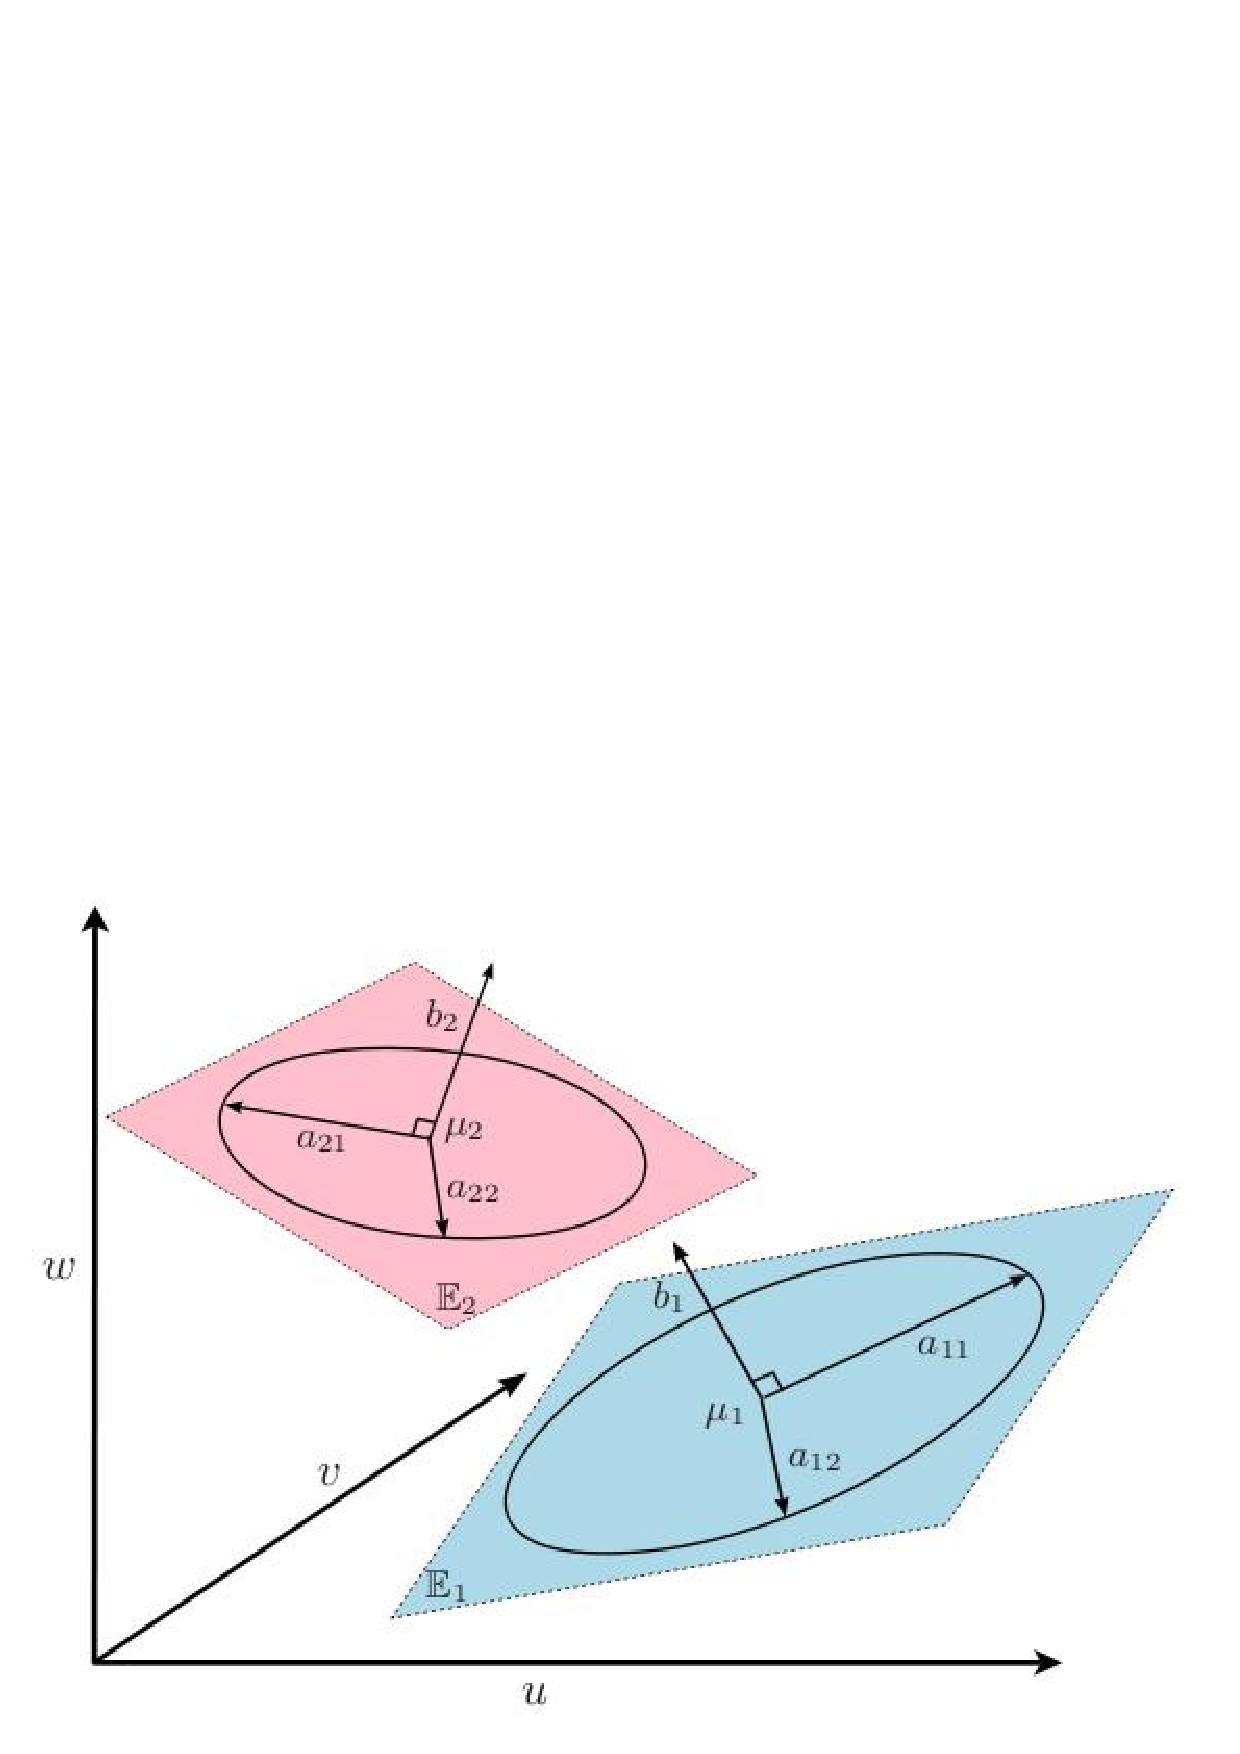
\includegraphics[scale=0.75]{Diagramme_1.epsi}
%  \end{center}
%  \caption{\label{cap:Illustration_model2}The parameters of the model
%    $[a_{kj}b_{k}D_{k}\delta_{k}]$ in the case of two classes.}
%\end{figure}



\begin{figure}[!ht]
  \centering
  \includegraphics[width=6.5cm, height=6cm]{Diagramme_1.eps}
  \caption{\label{cap:Illustration_model2}The parameters of the model $[a_{kj}b_{k}D_{k}\delta_{k}]$ in the case of two classes.}
 \end{figure}


\subsubsection{Sub-models of model $[a_{kj}b_{k}D_{k}\delta_{k}]$}
Starting from the general model $[a_{kj}b_{k}D_{k}\delta_{k}]$ and allowing the elements of the
model to vary or to be equal between classes, leads to 28 different models related to different
types of regularization. In {\sc mixmod} eight useful models have been selected:
\begin{itemize}
\item Two models with free dimension $\delta_k$:
  \begin{itemize}
  \item the model $[a_{kj}b_{k}D_{k}\delta_{k}]$
  \item the model $[a_{k}b_{k}D_{k}\delta_{k}]$
  \end{itemize}
\item Six models with fixed dimension $\delta$:
  \begin{itemize}
  \item the model $[a_{kj}b_{k}D_{k}\delta]$
  \item the model $[a_{j}b_{k}D_{k}\delta]$
  \item the model $[a_{kj}bD_{k}\delta]$
  \item the model $[a_{j}bD_{k}\delta]$
  \item the model $[a_{k}b_{k}D_{k}\delta]$
  \item the model $[a_{k}bD_{k}\delta]$
  \end{itemize}
\end{itemize}
Their main features are summarized in Table~\ref{cap:Some-properties-of-HDDA-models}. The
second column of this table gives the number of parameters to be estimated. The third column
provides the asymptotic order of the number of parameters to be estimated (with the assumption
$K\ll \delta_k\ll d$). The last column gives this number in the particular case $K=4$, $d=100$
and $\forall k,\, \delta_{k}=10$. These values are also given for the standard classification
methods QDA and LDA.  It is worthwhile to note that, in this cases, all HD models are more
parsimonious than both QDA and LDA.  Some particular situations lead to standard discriminant
methods. For example, if $\delta_{k}=(d-1)$, for $k=1,...,K$, the model reduces to
QDA. Moreover, if $a_{kj}=a_{j}$, $b_{k}=b$ and $D_{k}=D$, for $i=1,...,k$, it reduces to LDA.

\begin{table}
  \begin{center}\small{\begin{tabular}{lcccc}
        \hline
        Model&
        \begin{tabular}{c}
          Number of\tabularnewline
          parameters $n$\tabularnewline
        \end{tabular}&
        \begin{tabular}{c}
          Asymptotic\tabularnewline
          order\tabularnewline
        \end{tabular}&
        \begin{tabular}{c}
          Values of $n$ for $K=4$, \tabularnewline
          $p=100$ and $d=10$\tabularnewline
        \end{tabular}
        \tabularnewline
        \hline
        $[a_{kj}b_{k}D_{k}\delta_{k}]$ & $\rho+\bar{\tau}+2K+D$ & $Kd\delta$ & 4231
        \tabularnewline

        $[a_{k}b_{k}D_{k}\delta_{k}]$ & $\rho+\bar{\tau}+3K$ & $Kd\delta$ & 4195
        \tabularnewline
        \hline

        $[a_{kj}b_{k}D_{k}d]$ & $\rho+K(\tau+\delta+1)+1$ & $Kd\delta$ & 4228
        \tabularnewline

        $[a_{j}b_{k}D_{k}d]$ & $\rho+K(\tau+1)+\delta+1$ & $Kd\delta$ & 4198
        \tabularnewline

        $[a_{kj}bD_{k}d]$ & $\rho+K(\tau+\delta)+2$ & $Kd\delta$ & 4225
        \tabularnewline

        $[a_{j}bD_{k}d]$ & $\rho+K\tau+\delta+2$ & $Kd\delta$ & 4195
        \tabularnewline

        $[a_{k}b_{k}D_{k}d]$ & $\rho+K(\tau+2)+1$ & $Kd\delta$ & 4192
        \tabularnewline

        $[a_{k}bD_{k}d]$ & $\rho+K(\tau+1)+2$ & $Kd\delta$ & 4189
        \tabularnewline
        \hline

        QDA & $\rho+Kd(\delta+1)/2$ & $Kp^{2}/2$ & 20603
        \tabularnewline

        LDA & $\rho+\delta(\delta+1$)/2 & $p^{2}/2$ & 5453
        \tabularnewline
        \hline
      \end{tabular}}
  \end{center}
  \caption{\label{cap:Some-properties-of-HDDA-models}Features of the HD
    models: $\rho=Kd+K-1$ is the number of parameters required for the
    estimation of means and proportions, $\bar{\tau}=\sum_{k=1}^{K}\delta_{k}[p-(\delta_{k}+1)/2]$
    and $\tau=\delta[d-(\delta+1)/2]$ are the number of parameters required for
    the estimation of $\tilde{D_{k}}$ and $\tilde{D}$, and $D=\sum_{k=1}^{K}\delta_{k}$.
    For asymptotic order, it is assumed that $K\ll \delta\ll d$.}
\end{table}

\subsubsection{The MAP step}
The MAP decision rule for model $[a_{kj}b_{k}D_{k}\delta_{k}]$ yields to classify ${\bf x}$ in
class $C_{k^{*}}$ if $k^{*}=\argmin_{k=1,...,K}\{ \Gamma_{k}({\bf x})\}$ with
\begin{eqnarray*}
  \Gamma_{k}({\bf x})&=&\Vert\mu_{k}-P_{k}({\bf x})\Vert_{\mathcal{A}_{k}}^{2}
  +\frac{1}{b_{k}}\Vert {\bf x}-P_{k}({\bf x})\Vert^{2}\\
  &+& \sum_{j=1}^{\delta_{k}}\log(a_{kj})+(d-\delta_{k})\log(b_{k})-2\log(\pi_{k})+p\log(2\pi),
\end{eqnarray*}
$\Vert.\Vert_{\mathcal{A}_{k}}$ being a norm on $\mathbb{E}_k$ such that $\Vert {\bf x}
\Vert^{2}_{\mathcal{A}_{k}}={\bf x}^t\mathcal{A}_{k}{\bf x}$ with
$\mathcal{A}_{k}=\tilde{D_{k}}\Delta_{k}^{-1}\tilde{D_{k}}^{t}$.

This decision rule is based on two distances: the distance between the observation and the
subspace $\mathbb{E}_{k}$, and the distance between the projection of ${\bf x}$ on
$\mathbb{E}_{k}$ and the mean of the class. It also depends on the variances $a_{kj}$ and
$b_{k}$ and on prior probabilities $\pi_{k}$. Figure~\ref{cap:Illustration_model} depicts the
decision rule.  It illustrates the fact the projection on $\mathbb{E}_{k}^{\perp}$ is not
required, reducing dramatically the number of parameters to be estimated and avoiding numerical
difficulties.

\begin{figure}[]
  \begin{center}\psfrag{Ei}{\footnotesize$E_k$}
    \psfrag{xx}{\footnotesize$x$}
    \psfrag{Pi}{\footnotesize$P_k(x)$}
    \psfrag{mu}{\footnotesize$\mu_k$}
    \psfrag{d_1}{\footnotesize$d(x,E_k)$}
    \psfrag{d2}{}
    \psfrag{d3}{\footnotesize$d(\mu_k,P_k(x))$}
    \psfrag{Ei_perp}{\footnotesize${E_k}^\perp$}
    \psfrag{Pi_perp}{\hspace{-2ex}\footnotesize${P_k}^\perp(x)$}
    \includegraphics[scale=0.55]{illustration_1.eps}
  \end{center}
  \caption{\label{cap:Illustration_model}The subspaces $\mathbb{E}_{k}$ and
    $\mathbb{E}_{k}^{\perp}$ of the class $C_{k}$.}
\end{figure}


\subsubsection{Estimation of the model parameters}
The parameters of the mixture of factor analyzers models are estimated through the maximum
likelihood approach.  Estimation of parameters $\pi_{k}$ and $\mu_{k}$ of class $C_{k}$ are
\[\hat{\pi}_{k}=\frac{n_{k}}{n},\,\hat{\mu}_{k}=\frac{1}{n_{k}}\sum_{{\bf x}_{k}\in C_{k}}{\bf x}_{j}.\]
In what follows, we make use of $W_k=\sum_{{\bf x}_{j}\in C_{k}}({\bf
  x}_{j}-\hat{\mu}_{k})^{t}({\bf x}_{j}-\hat{\mu}_{k})$, $n_{k}=\mbox{card}(C_{k})$,
$W=\sum_{i=k}^{K}\hat{\pi}_{k}W _{k}$, $\lambda_{kj}$ which denotes the $j$th largest
eigenvalue of $W_{k}$ and $\lambda_{j}$ the $j$th largest eigenvalue of $W$, to define the
m.l. estimate of the mixture component variance that are now presented.  Details can be found
in Bouveyron {\it et al.} (2007).

\paragraph{Models with free $\delta_k$}
Assuming that dimensions $\delta_{k}$ are known for $k=1,...,K$, the following closed form
estimators of model parameters are derived.

\paragraph{Subspace $\mathbb{E}_{k}$} The $\delta_{k}$ first columns
of $D_{k}$ are estimated by the eigenvectors associated with the
$\delta_{k}$ largest eigenvalues $\lambda_{kj}$ of $W_{k}$.

\paragraph{Model $[a_{kj}b_{k}D_{k}\delta_{k}]$}
The estimators of $a_{kj}$ are the $\delta_{k}$ largest eigenvalues $\lambda_{kj}$ of $W_{k}$
divided by $n_k$ and
\begin{equation}
  \hat{b}_{k}=\frac{1}{n_k(d-\delta_{k})}\left(\tr(W_{k})-\sum_{j=1}^{\delta_{k}}\lambda_{kj}\right).
  \label{eq:estimator_of_b_i_d_i}
\end{equation}

\paragraph{Model $[a_{k}b_{k}D_{k}\delta_{k}]$}
The estimator of $b_{k}$ is given by (\ref{eq:estimator_of_b_i_d_i}) and
\begin{equation}
  \hat{a}_{k}=\frac{1}{n_k\delta_{k}}\sum_{j=1}^{\delta_{k}}\lambda_{kj},
  \label{eq:estimator_of_a_i_di}
\end{equation}

\paragraph{Models with common $\delta_k$}
Assuming that parameter $\delta$ is known, we obtain the following closed form estimators for
the parameters of the models with common $\delta_k$, equal to $\delta$.

\paragraph{Subspace $\mathbb{E}_{k}$}
The $\delta$ first columns of $D_{k}$ are estimated by the eigenvectors associated with the
$\delta$ largest eigenvalues $\lambda_{kj}$ of $W_{k}$.

\paragraph{Model $[a_{kj}b_{k}D_{k}d]$}
The estimators of $a_{kj}$ are the $\delta$ largest eigenvalues $\lambda_{kj}$ of $W_{k}$
divided by $n_k$ and
\begin{equation}
  \hat{b}_{k}=\frac{1}{n_k(d-\delta)}\left(\tr(W_{k})-\sum_{j=1}^{d}\lambda_{kj}\right).
  \label{eq:estimator_of_b_i_d}
\end{equation}

\paragraph{Model $[a_{j}b_{k}D_{k}d]$}
The estimator of $b_{k}$ is given by~(\ref{eq:estimator_of_b_i_d}) and
\begin{equation}
  \hat{a}_{j}=\frac{1}{n}\sum_{k=1}^{K}\hat{\pi}_{k}\lambda_{kj}.
  \label{eq:estimator_of_a_j_d}
\end{equation}

\paragraph{Model $[a_{kj}bD_{k}d]$}
The estimators of $a_{kj}$ are the $\delta$ largest eigenvalues $\lambda_{kj}$ of $W_{k}$
divided by $n_k$ and
\begin{equation}
  \hat{b}=\frac{1}{n(d-\delta)}\left(\tr(W)-\sum_{k=1}^{K}\hat{\pi_k}\sum_{j=1}^{d}\lambda_{kj}\right).
  \label{eq:estimator_of_b_d}
\end{equation}

\paragraph{Model $[a_{j}bD_{k}d]$}
The estimators of $a_j$ are given by~(\ref{eq:estimator_of_a_j_d}) and the estimator of~$b$ is
given by~(\ref{eq:estimator_of_b_d}).

\paragraph{Model $[a_{k}b_{k}D_{k}d]$}
The estimator of $b_{k}$ is given by (\ref{eq:estimator_of_b_i_d}) and
\begin{equation}
  \hat{a}_{k}=\frac{1}{nd}\sum_{j=1}^{d}\lambda_{kj},
  \label{eq:estimator_of_a_i_d}
\end{equation}

\paragraph{Model $[a_{k}bD_{k}d]$}
The estimator of $a_{k}$ is given by~(\ref{eq:estimator_of_a_i_d}) and the estimator of $b$ is
given by~(\ref{eq:estimator_of_b_d}).

\paragraph{Estimation of intrinsic dimensions}
The last parameters to be estimated are the intrinsic dimensions $\delta_k$ of the $K$
classes. It is not possible to estimate the dimensions $\delta_k$ using the maximum likelihood
approach and minimizing the cross validated error rate is considered.  However, this
minimization technique is not implemented in the present version of {\sc mixmod} and the user
has to provide all the intrinsic dimensions~$\delta_k$.


%%%%%%%%%%%%%%%%%%%%%%%%%%%%%%%%%%%%%%%%%%%%%%%%%%%%%%%%%%%%%%%%%%%%%%%%%%%%%%%%%%%%%%%%%%%%%
%%%%%%%%%%%%%%%%%%%%%%%%%%%%%%%%%%%%%%%%%%%%%%%%%%%%%%%%%%%%%%%%%%%%%%%%%%%%%%%%%%%%%%%%%%%%%
%%%%%%%%%%%%%%%%%%%%%%%%%%%%%%%%%%%%%%%%%%%%%%%%%%%%%%%%%%%%%%%%%%%%%%%%%%%%%%%%%%%%%%%%%%%%%
\section{The multinomial mixture model}
\subsection{Definition}
We consider now that data are $n$ objects described by $d$ categorical variables, with
respective number of categories $m_1,\ldots,m_d$, so ${\mathcal X}=\{1,\ldots,m_1\}\times\ldots\times\{1,\ldots,m_d\}$. The data can be represented by $n$ binary
vectors ${\bf x}_i = (x_i^{jh} ; j=1,\ldots,d; h = 1,\ldots,m_j)$ ($i=1,\ldots,n$) where
$x_i^{jh}=1$ if the object $i$ belongs to the category $h$ of the variable $j$ and 0 otherwise.
Denoting $m=\sum_{j=1}^dm_j$ the total number of categories, the data are defined by the matrix
${\bf x} = ({\bf x}_1,\ldots,{\bf x}_n)$ with $n$ rows and $m$ columns.  Binary data can be
seen as a particular case of categorical data with $d$ dichotomous variables, i.e.  $m_j=2$ for
any $j=1,\ldots,d$.

The latent class model assumes that the $d$ categorical variables are independent given the latent
variable. Formulated in mixture terms (Everitt 1984), each ${\bf x}_i$ arises independently
from a mixture of multivariate multinomial distributions defined by
\begin{eqnarray}
  f(\bx_i|\theta) = \sum_{k=1}^K p_k h(\bx_i|\balpha_k)
\end{eqnarray}
where $p_k$ is the mixing proportion ($0<p_k<1$ for all $k=1,...,K$ and $p_1+...+p_K=1$) of the
$k$th component and where, for $k=1,\ldots,K$,
\begin{equation}
  \label{eq:hmulti}
  h(\bx_i|\balpha_k) = \prod_{j=1}^d \prod_{h=1}^{m_j} (\alpha_k^{jh})^{x_i^{jh}}
\end{equation}
with $\balpha_k = (\alpha_k^{jh};j=1,\ldots,d;h=1,\ldots,m_j)$. In (\ref{eq:hmulti}), we
recognize the product of $d$ conditionally independent multinomial distributions of parameters
$\balpha_k^j$.  The mixture parameters is denoted by
$\theta=\left(p_1,\ldots,p_{K-1},\balpha_1,\ldots,\balpha_K\right)$.

This model may present problems of identifiability (see for instance Goodman 1974) but most
situations of interest are identified.

%%%%%%%%%%%%%%%%%%%%%%%%%%%%%%%%%%%%%%%%%%%%%%%%%%%%%%%%%%%%%%%%%%%%%%%%%%%%%%%%%%%%%%%%%%%%%
\subsection{Five multinomial models}
In order to propose more parsimonious models than the previous one, we present the following
extension of the parameterization of Bernoulli distributions used by Celeux and Govaert (1991)
for clustering and also by Aitchison and Aitken (1976) for kernel discriminant analysis.

The basic idea is to impose the vector $\balpha_k^j = (\alpha_k^{j1},\ldots,\alpha_k^{jm_j})$
to take the form $(\beta_k^j,\ldots,\beta_k^j,\gamma_k^j,\beta_k^j,\ldots,\beta_k^j)$ with
$\gamma_k^j > \beta_k^j$. Since $\sum_{h=1}^{m_j} \alpha_k^{jh}=1$, we have
$(m_j-1)\beta_k^j+\gamma_k^j = 1$ and, consequently, $\beta_k^j=(1-\gamma_k^j)/(m_j-1)$. The
constraint $\gamma_k^j>\beta_k^j$ becomes finally $\gamma_k^j > 1 /m_j$.  Then, the vector
$\balpha_k^j$ can be broken up into the two following parameters:
\begin{itemize}
\item ${\bf a}_k^j = (a_k^{j1},\ldots,a_k^{jm_j})$ where $a_k^{jh} = 1$ if $h$ corresponds to
  the rank of $\gamma_k^j$ (in the following, this rank will be noted $h(k,j)$), 0 otherwise;
\item $\varepsilon_k^j = 1 - \gamma_k^j$ which corresponds to the probability that the data
  ${\bf x}_i$ arising from the $k$th component are such that $x_i^{jh(k,j)} \neq 1$.
\end{itemize}
In other words, the multinomial distribution associated to the $j$th variable of the $k$th
component is reparameterized by a center ${\bf a}_k^j$ and the dispersion $\varepsilon_k^j$
around this center. Thus, it allows us to give an interpretation similar to the center and the
variance matrix used for continuous data in the Gaussian mixture context.

Since, the relationship between the initial parameterization and the new one is given by:
\begin{equation}
  \alpha_k^{jh} = \left\{
    \begin{array}{ll}
      1-\varepsilon_k^j & \mbox{if $h=h(k,j)$} \\
      \varepsilon_k^j / (m_j-1) & \mbox{otherwise,}
    \end{array}
  \right.
\end{equation}
Equation (\ref{eq:hmulti}) can be rewritten with ${\bf a}_k = ({\bf a}_k^j ;
j=1,\ldots,d)$ and $\bvarepsilon_k = (\varepsilon_k^j ; j=1,\ldots,d)$
\begin{equation}
  h(\bx_i|\balpha_k) = \tilde h(\bx_i|{\bf a}_k,\varepsilon_k) =
  \prod_{j=1}^d \prod_{h=1}^{m_j} \left(
    (1-\varepsilon_k^j)^{a_k^{jh}} (\varepsilon_k^j /
    (m_j-1))^{1-a_k^{jh}} \right)^{x_i^{jh}}.
\end{equation}
In the following, this model will be denoted by $[\varepsilon_k^j]$. In this context, three
other models can be easily deduced. We note $[\varepsilon_k]$ the model where $\varepsilon_k^j$
is independent of the variable $j$, $[\varepsilon^j]$ the model where $\varepsilon_k^j$ is
independent of the component $k$ and, finally, $[\varepsilon]$ the model where
$\varepsilon_k^j$ is independent of both the variable $j$ and the component $k$.  In order to
maintain some unity in the notation, we will denote also $[\varepsilon_k^{jh}]$ the most
general model introduced at the previous section.  The number of free parameters associated to
each models is given in Table~\ref{tab:model.multi}.

\begin{table}[hbtp]
  \begin{center}
    \begin{tabular}{|c|c|}
      \hline model & number of parameters \\
      \hline $[\varepsilon]$ & $\delta + 1$ \\
      $[\varepsilon^j]$ & $\delta + d$ \\
      $[\varepsilon_k]$ & $\delta + K$ \\
      $[\varepsilon_k^j]$ & $\delta + Kd$ \\
      $[\varepsilon_k^{jh}]$ & $\delta + K \sum_{j=1}^d (m_j-1)$ \\
      \hline
    \end{tabular}
  \end{center}
  \caption{Number of free parameters of the five multinomial models. We have
    $\delta=K-1$ in the case of free proportions and $\delta=0$ in
    the case of equal proportions.} \label{tab:model.multi}
\end{table}

%%%%%%%%%%%%%%%%%%%%%%%%%%%%%%%%%%%%%%%%%%%%%%%%%%%%%%%%%%%%%%%%%%%%%%%%%%%%%%%%%%%%%%%%%%%%%
\subsection{M step for each of the five models}
The M step has to be detailed for each of the five models presented above. Using notation
already defined in the Gaussian mixture context, the M step consists of maximizing in $\theta$
the function:
\begin{equation}
  F(\theta| {\bf x}, {\bf
    c})=\sum_{i=1}^{n}\sum_{k=1}^{K} c_{ik} \ln \left [p_{k}  h({\bf
      x}_{i}|\balpha_{k})\right ] \label{eq:Mstep.multi}
\end{equation}
for fixed {\em classification} matrix ${\bf c}$ (obtained at the previous E or S or C steps)
and with data matrix ${\bf x}$. We now detail the m.l. estimations of the parameters
$\balpha_1,\ldots,\balpha_K$ of the multinomial distributions. In the following, we adopt the
notation $e_k^{jh} = n_k - \sum_i c_{ik}x_i^{jh}$ and also $h(k,j)$ for the value of $h$ which
minimizes $e_k^{jh}$. In other terms, $h(k,j)$ still denotes the rank of the modality which
occurs the most frequently for a given variable $j$ and a given component $k$. For convenience,
we use also $e_k^j = e_k^{jh(k,j)}$.

\paragraph{Model $[\varepsilon_k^{jh}]$}
\begin{equation}
  \alpha_k^{jh} = 1 - e_k^{jh} / n_k.
\end{equation}

\paragraph{Model $[\varepsilon_k^j]$}
\begin{equation}
  \alpha_k^{jh} =
  \left\{
    \begin{array}{ll}
      1-e_k^j / n_k & \mbox{if $h=h(k,j)$} \\
      e_k^j / (n_k(m_j-1)) & \mbox{otherwise.}
    \end{array}
  \right.
\end{equation}

\paragraph{Model $[\varepsilon_k]$}
\begin{equation}
  \alpha_k^{jh} =
  \left\{
    \begin{array}{ll}
      1-(\sum_j e_k^j) / (n_k d) & \mbox{if $h=h(k,j)$} \\
      (\sum_j e_k^j) / (n_k d(m_j-1)) & \mbox{otherwise.}
    \end{array}
  \right.
\end{equation}

\paragraph{Model $[\varepsilon^j]$}
\begin{equation}
  \alpha_k^{jh} =
  \left\{
    \begin{array}{ll}
      1-(\sum_k e_k^j) / n & \mbox{if $h=h(k,j)$} \\
      (\sum_k e_k^j) / (n(m_j-1)) & \mbox{otherwise.}
    \end{array}
  \right.
\end{equation}

\paragraph{Model $[\varepsilon]$}
\begin{equation}
  \alpha_k^{jh} =
  \left\{
    \begin{array}{ll}
      1-(\sum_{j,k} e_k^j) / (nd) & \mbox{if $h=h(k,j)$} \\
      (\sum_{j,k} e_k^j) / (nd(m_j-1)) & \mbox{otherwise.}
    \end{array}
  \right.
\end{equation}

\paragraph{Using the new parameterization}
In fact, we could prefer to express the M step with the new parameterization ${\bf a}_k$ and
$\bvarepsilon_k$ (for models $[\varepsilon_k^j]$, $[\varepsilon_k]$, $[\varepsilon^j]$ and
$[\varepsilon]$) instead of $\balpha_k$, in particular for the meaningful interpretation of the
terms ${\bf a}_k$ and $\bvarepsilon_k$. In this case, it is easy to deduce expressions of ${\bf
  a}_k$ and $\bvarepsilon_k$ from the expressions given above for $\balpha_k$ with the
following relationships:
\begin{equation}
  a_k^{jh} =
  \left\{
    \begin{array}{ll}
      1 & \mbox{if $h=h(k,j)$} \\
      0 & \mbox{otherwise,}
    \end{array}
  \right.
\end{equation}
and
\begin{equation}
  \varepsilon_k^j = 1 - \alpha_k^{jh(k,j)}.
\end{equation}

\section{The Gaussian-multinomial mixture model}

\subsection{Definition}

We consider now that data are $n$ objects described by $d$ variables mixing $d^{(q)}$ quantitative variables and $d^{(c)}$ categorical variables with respective number of categories $m_1,\ldots,m_{d^{(c)}}$. Thus, ${\mathcal X}=\IR^{d^{(q)}}\times\{1,\ldots,m_1\}\times\ldots\times\{1,\ldots,m_{d^{(c)}}\}$, with $d=d^{(q)}+d^{(c)}$. Each individual can be written $\bx_i=(\bx_i^{(q)},\bx_i^{(c)})$, where $\bx_i^{(q)}\in \IR^{d^{(q)}}$ and $\bx_i^{(c)}\in \{1,\ldots,m_1\}\times\ldots\times\{1,\ldots,m_{d^{(c)}}\}$ denote respectively the quantitative and the categorical parts of $\bx_i$.

The latent class model (Everitt 1984) is assumed for {\em all} $d$ variables which means that the $d$ variables (quantitative and categorical) are independent given the latent variables. Restricting not only categorical variables but also quantitative ones to be independent avoids to favor information provided by quantitative variables in the estimation process. Formulated in mixture terms, each $\bx_i$ arises independently from a mixture of combined multivariate {\em diagonal} Gaussian and
multivariate distribution defined by
\begin{eqnarray}
  f(\bx_i|\theta) & = & \sum_{k=1}^K p_k h(\bx_i|\blambda_k) \\
  & = & \sum_{k=1}^K p_k \left\{h^{(q)}(\bx_i^{(q)}|\bmu_k) + h^{(c)}(\bx_i^{(c)}|\balpha_k) \right\},
\end{eqnarray}
where
\begin{itemize}
\item $\blambda_k=(\bmu_k,B_k,\balpha_k)$.
\item $h^{(q)}(\cdot|\bmu_k,B_k)$ is a $d^{(q)}$ dimensional Gaussian density of center $\bmu_k$ and {\em diagonal} variance matrix $B_k$ (see Section~5.1).
\item $h^{(c)}(\cdot|\balpha_k)$ is a $d^{(c)}$ dimensional multivariate distribution of parameter $\balpha_k$ (see Section~6.1).
\end{itemize}
The whole mixture parameter is denoted by
\[
\theta=(p_1,\ldots,p_{K-1},\bmu_1,\ldots,\bmu_K,B_1,\ldots,B_K,\balpha_1,\ldots,\balpha_K).
\]

\subsection{Thirty combined Gaussian-multinomial models}

In order to propose more parsimonious models than the previous ones, one may combine the four Gaussian diagonal models $[\lambda B]$, $[\lambda_k B]$, $[\lambda B_k]$, $[\lambda_k B_k]$ or the two spherical Gaussian models $[\lambda I]$, $[\lambda_k I]$ respectively defined in Section~5.2.3 and~5.2.4 with the five multivariate multinomial models $[\varepsilon]$, $[\varepsilon^j]$, $[\varepsilon_k]$, $[\varepsilon_k^j]$, $[\varepsilon_k^{jh}]$ defined in Section~6.2. It leads to considering 30 different combined Gaussian-multinomial models. For instance, the Gaussian-multinomial model denoted by $[\lambda B,\varepsilon]$ indicates a combination of the Gaussian model $[\lambda B]$ and of the multinomial model $[\varepsilon]$, and so on.

\subsection{M step for the 30 models}

The M step has to be performed independently for the multivariate Gaussian and for the multivariate multinomial distributions:
\begin{itemize}
\item For the Gaussian part, use the M step in Section~5.3 to estimate all $\bmu_k$ and $B_k$ which correspond to the Gaussian model at hand.
\item For the multinomial part, use the M step in Section~6.3 to estimate all $\balpha_k$ which correspond to the multinomial model at hand.
\end{itemize}

\newpage
\part*{References}
\addcontentsline{toc}{part}{Selected references}
\markboth{Selected references}{}
\begin{description}
\item[    ] Aitchison, J. and Aitken, C. G. G. (1976), ``Multivariate Binary Discrimination by the Kernel Method,"
{\em Biometrika}, {\em 63}, 413-420.
%\item[    ] Aitkin, M. and Rubin, D. B. (1985), ``Estimation and Hypothesis
%Testing in Finite Mixture Models," {\em Journal of the Royal
%Statistical Society}, Series B, {\em 47}, 67-75.
%\item[    ] Aitkin, M. and Tunnicliffe Wilson, G. (1980), ``Mixture Models,
%Outliers and the EM Algorithm," {\em Technometrics}, {\em 22}, 325-332.
%\item[    ] Akaike, H. (1974), ``A New Look at the Statistical
%Identification Model," {\em IEEE Transactions on Automatic Control}, {\em 19}, 716-723.
\item[    ] Banfield, J. D. and Raftery, A. E. (1993), ``Model-Based
Gaussian and non Gaussian Clustering," {\em Biometrics,} {\em 49}, 803-821.
%\item[    ] Bensmail, H. and Celeux G. (1996), ``Regularized Gaussian discriminant analysis through eigenvalue decomposition''. Journal of the American Statistical Association, {\em 91}, 1743-48.
%\item[    ] Bezdek, J. C. (1981), {\em Pattern Recognition with Fuzzy
%Objective Function Algorithms}, New York: Plenum.
\item[    ] Biernacki, C. Celeux, G. and Govaert, G. (1999), ``An improvement of the NEC criterion for assessing the number of components arising from a mixture,''
{\em Pattern Recognition letters}, No 20, 267-272.
\item[    ] Biernacki, C. and Govaert, G. (1999). Choosing Models in Model-based Clustering and Discriminant Analysis.
{\em Journal of Statistical Computation and Simulation, 64, 49-71}.
\item[    ] Biernacki, C. Celeux, G. and Govaert, G. (2000), ``Assessing a Mixture Model for Clustering with the Integrated Completed Likelihood,"
{\em IEEE Transactions on Pattern Analysis and Machine Intelligence}, vol {\em 22}, No 7, 719-725.
\item[    ] Biernacki, C. Celeux, G. and Govaert, G. (2003) "Choosing starting values for the EM algorithm for getting the highest
likelihood in multivariate Gaussian mixture models''. {\em Computational Statistics and Data Analysis}, {\em 41}, 561-575.
%\item[    ] Bock, H. H. (1985), ``On Tests Concerning the Existence of a
%Classification," {\em Journal of Classification}, {\em 2}, 77-108.
%\item[    ] Bock, H. H. (1989), ``Probabilistic Aspects in Cluster
%Analysis," in {\em Conceptual and Numerical Analysis of Data}, O. Opitz (ed.)
%Springer-Verlag, Heidelberg, pp. 12-44.
\item[    ] Bouveyron C., Girard S. and Schmid C., High Dimensional Discriminant Analysis, {\em Communications in Statistics:
Theory and Methods, 36}, 2607-2623.
%\item[    ] Bozdogan, H. (1990), ``On the Information-Based Measure of
%Covariance Complexity and its Application to the Evaluation of
%Multivariate Linear Models," {\em Communications in Statistics, Theory
%and Methods} {\em 19}, 221-278.
\item[    ] Bozdogan, H. (1993), ``Choosing the Number of Component Clusters in the
Mixture-Model Using a New Informational Complexity Criterion of the
Inverse-Fisher Information Matrix," in {\em Information and Classification},
O. Opitz, B. Lausen, and R.
Klar (eds.), Heidelberg: Springer-Verlag,  pp. 40-54.
%\item[    ] Bozdogan, H. and Sclove, S. L. (1984), ``Multi-Sample Cluster
%Analysis using Akaike 's Information Criterion," {\em Annals of Institute
%of Statistical Mathematics}, {\em 36}, 163-180.
%\item[    ] Bryant, P. G. (1991), ``Large-Sample Results for
%Optimization Based Clustering Methods," {\em Journal of
%Classification}, {\em 8}, 31-44.
%\item[    ] Bryant, P. G. (1993), ``On Detecting the Numbers of Clusters
%Using the MDL Principle,"
%Unpublished Manuscript.
%\item[    ] Bryant, P. G. and Williamson, J. A. (1978), ``Asymptotic Behavior
%of Classification Maximum Likelihood Estimates," {\em Biometrika}, {\em 65}, 273-281.
%\item[    ] Bryant, P. G. and Williamson, J. A. (1986), ``Maximum Likelihood
%and Classification: a Comparison of Three Approaches," in
%{\em Classification as a tool of research}, W. Gaul and M. Schader (eds.)
%North-Holland,   pp. 33-45.
%\item[    ] Celeux G. and Diebolt J. (1985) "The SEM algorithm : a probabilistic teacher algorithm derived from the EM algorithm for the mixture problem". {\em Comp. Statis. Quaterly, 2, 73-82}.
%\item[    ] Celeux, G. (1986), ``Validity Tests in Cluster Analysis
%Using a Probabilistic Teacher Algorithm," {\em COMPSTAT 90}, F. de Antoni, N. Lauro and A. Rizzi
%(eds.)
%Heidelberg: Springer-Verlag, pp. 163-169.
\item[    ] Celeux, G. and Govaert, G. (1991), ``Clustering Criteria for Discrete
Data and Latent Class Models," {\em Journal of Classification}, {\em 8}, 157-176.
\item[    ] Celeux, G. and Govaert, G. (1992). A classification EM
algorithm for clustering and two stochastic versions. {\em
Computational Statistics \& Data Analysis}, {\bf 14}, 315-332.
%\item[    ] Celeux, G. and Govaert, G. (1993), ``Comparison of the Mixture
%and the Classification Maximum Likelihood in Cluster Analysis,"
%{\em Journal of Statistical Computation and Simulation}, {\em 47}, 127-146.
\item[    ]  Celeux, G. and Govaert, G. (1995) "Parsimonious Gaussian models in cluster analysis". {\em Pattern Recognition, 28, 781-793}.
\item[    ] Celeux, G. and Soromenho, G. (1996) "An entropy criterion for assessing the number of clusters in a mixture model". {\em Journal of Classification, 13, 195-212}.
%\item[    ] Culter, A. and Windham, M. P. (1993), ``Information-Based
%Validity Functionals for Mixture Analysis," {\em Proceedings of the
%first US-Japan Conference on the Frontiers of Statistical Modeling.}
%(H. Bozdogan ed.),  Amsterdam: Kluwer, pp. 149-170.
\item[    ] Dempster, A. P., Laird, N. M. and Rubin, D. B. (1977). Maximum likelihood from incomplete data via the EM algorithm (with discussion). {\em J. R. Statis. Soc. B}, {\bf 39}, 1-38.
\item[    ] Everitt, B. (1984). {\em An Introduction to Latent Variable Models}. London,
Chapman and Hall.
\item[    ] Fraley, C. and Raftery, A. E. (1998): How Many Clusters ? Answers
via Model-based Cluster Analysis. {\em The Computer Journal, 41}, 578-588.
215-231.
%\item[    ] Flury, B. W. (1984). Common principal components in $k$ groups. {\em JASA}, {\bf 79}, 892-897.
\item[    ] Flury, B. W., Gautschi, W. (1986). An algorithm for simultaneous orthogonal transformation of several positive
definite symmetric matrices to nearly diagonal form. {\em SIAM J. Scientific Statist. Comput.}, {\bf 7}, 169-184.
%\item[    ] Flury, B. W., Schmid, M. J. and Narayanan, A. (1993) Error rates in quadratic
%discrimination with contraints on the covariance matrices. {\em Journal of Classification} (to appear).
\item[    ] Friedman, H. P. and Rubin, J. (1967). On some invariant
criteria for grouping data. {\em JASA,} {\bf 62}, 1159-1178.
%\item[    ] Ganesalingam, S. (1989), ``Clasification
%and Mixture Approaches to Clustering via Maximum Likelihood," {\em
%Applied Statistics}, {\em 38}, 455-466.
\item[    ] Goodman, L. A. (1974), ``Exploratory Latent Structure Analysis Using Both Identifiable and Unidentifiable Models," {\em Biometrika}, {\em 61},
%\item[    ] Hathaway, R. J. (1986), ``Another Interpretation of the EM
%Algorithm for Mixture Distributions," {\em Statistics and Probability
%Letters}, {\em 4}, 53-56.
\item[    ] Keribin, C. (2000). Consistent estimation of the order of mixture.
{\em Sankhya}, {\em 62}, 49-66.
%\item[    ] Koehler, A. B. and Murphree, E. H. (1988), ``A Comparison of
%the Akaike and Schwarz Criteria for Selecting Model Order," {\em
%Applied Statistics}, {\em 37}, 187-195.
%\item[    ] Macqueen, J. (1967), ``Some Methods for Classification and
%Analysis of Multivariate Observations," {\em Proceedings of the 5th
%Berkeley Symposium on Mathematical Statistics and Probability},
%L. M. Le Cam and J. Neyman (eds.), Berkeley: University of California Press, Vol. 1 pp. 281-297.
\item[    ] Maronna, R. and Jacovkis, P. M. (1974). Multivariate procedures with variable metrics. {\em Biometrics}, {\bf 30}, 499-505.
%\item[    ] Marriott, F. H. C. (1975), ``Separating Mixtures of Normal Distributions,''
%{\em Biometrics, 31}, 767-769.
%\item[    ] Marriott, F. H. C. (1982). Optimization methods of cluster analysis. {\em Biometrika}, {\bf 69}, 239-249.
%\item[    ] McLachlan, G. J. (1987), ``On Bootstraping the Likelihood
%Ratio Test Statistic for the Number of Components in a Normal Mixture,"
%{\em Applied Statistics} {\em 36}, 318-324.
\item[    ] McLachlan, G. J. (1982). The classification and mixture maximum likelihood approaches to cluster analysis.
in {\em Handbook of Statistics} (Vol. 2), P. R. Krishnaiah and L. N. Kanal (Eds.). Amsterdam: North-Holland, pp. 199-208.
%\item[    ] McLachlan, G. J. and Basford K. E. (1989). {\em Mixture
%Models, Inference and Applications to Clustering}. New
%York, Marcel Dekker.
\item[    ] McLachlan, G. J. and Peel D. (2000). {\em Finite Mixture Models}. New York, Wiley.
\item[    ] McNicholas, P.D. and Murphy, T.B. (2008) Parsimonious Gaussian Mixture Models. {\em Statistics and Computing}, to appear.
%\item[    ] Rissanen, J. (1989),  {\em Stochastic Complexity  in
%Statistical Inquiry}, Teaneck,
%New Jersey: World Scientific.
\item[    ] Schwarz, G. (1978), ``Estimating the Dimension of a Model,"
{\em Annals of Statistics}, {\em 6}, 461-464.
\item[    ] Scott, A. J. and Symons, M. J. (1971). Clustering methods
based on likelihood ratio criteria. {\em Biometrics}, {\bf 27}, 387-397.
%\item[    ] Soromendho, G. (1994), ``Comparing Approaches for Testing the
%Number of Components in a Finite Mixture Model," {\em Computational
%Statistics, 9,} 65-78.
%\item[    ] Symons, M. J. (1981). Clustering criteria and multivariate normal mixtures. {\em Biometrics}, {\bf 37}, 35-43.
\item[    ] Tipping, M. E. and C. M. Bishop (1999). Mixtures of probabilistic principal component analysers. N{\em eural Computation  11}, 443-482.
%\item[    ] Titterington, D. M., Smith, A. F., and Markov, U. E. (1985),
%{\em Statistical Analysis of Finite Mixture Distributions}, New York: Wiley.
\item[    ]Ward, J.H. (1963) Hierarchical groupings to optimize an objective function. {\em JASA}, {\bf 58}, 236-244.
%\item[    ] Windham, M. P. and Cutler, A. (1992), ``Information Ratios
%for Validating Cluster Analyses," {\em Journal of the American
%Statistical Association}, {\em 87}, 1188-1192.
%\item[    ] Wolfe, J. H. (1970), ``Pattern Clustering by Multivariate
%Mixture Analysis," {\em Multivariate Behavioral Research}, {\em 5}, 329-350.
%\item[    ] Wolfe, J. H. (1971), ``A Monte Carlo Study of the Sampling Distribution
%of the Likelihood Ratio for Mixtures of Multinormal
%Distributions," US Naval Personnel Research Activity.
%{\em Technical Bulletin} {\em STB 72-2}, San Diego, California.
\end{description}

%%%%%%%%%%%%%%%%%%%%%%%%%%%%%%%%%%%%%%%%%%%%%%%%%%%%
\end{document}
